\documentclass[normalheadings,tablecaptionabove,twoside,openright,chapterprefix,halfparskip,fontsize=10pt,numbers=noenddot]{scrbook} %b5,17cm:24cm,BCOR=1cm

%%%%%%%
%Language
%%%%%%%
\usepackage[british]{babel}
\usepackage[applemac]{inputenc}
\usepackage[T1]{fontenc}

%%%%%%%
%Figures
%%%%%%%
\usepackage{graphicx}								%include pictures, diagrams, or drawings
\usepackage[small, bf, up, hang]{caption}					%customization of captions
%\usepackage[percent]{overpic}						%enables Latex constructs over graphics

%%%%%%%
%Tables
%%%%%%%
\usepackage{booktabs}								%enhance the quality of your tables by new line commands replacing \hline and \cline
\usepackage{multirow}
\usepackage{rotating}								%pro?vi?des the side?ways environ?ment; rotate a whole table by using the side?waysta?ble instead of the table environment
\usepackage{threeparttable}							%package facilitates tables with titles (captions) and notes
\usepackage{longtable}

%%%%%%%
%Math
%%%%%%%
\usepackage{amsmath}								%com?mands and environ?ments for maths
\usepackage{nicefrac}								%nice?frac com?mand, which crea?tes a frac?tion with dia?go?nal frac?tion line
\usepackage{units}									%com?mands unit[2.3]{N} and unitfrac[4.3]{Nm}{s} for nicely set units.
\usepackage{textgreek}
\usepackage{textcomp}

%%%%%%%
%Bibliography
%%%%%%%
\usepackage{natbib} %careful with this one, it makes the bibliography work. Include this to use the apalike style!

\usepackage{url}

%%%%%%%
%Miscellaneous
%%%%%%%
\usepackage{lscape}

\usepackage{microtype}
\usepackage[defaultlines=2,all]{nowidow}

\usepackage{xspace}

\usepackage{helvet}

\usepackage{lipsum}

\usepackage{layout}

\usepackage{setspace}
\onehalfspacing

\usepackage[usenames,dvipsnames,table]{xcolor}							%coloring columns, rows, single entries, and lines in many ways

\usepackage{fancyhdr}								%loads 'fancy' page style to allow customisation of header and footer
\fancyhf{}
\fancyhead[LE]{\small\nouppercase{\leftmark}}
\fancyhead[RO]{\small\nouppercase{\rightmark}}
\fancyfoot[LE,RO]{\thepage}

\fancypagestyle{plain}{%redefining plain pagestyle
	\fancyfoot[LE,RO]{\thepage} %prints the page number on the right side of the header
	\renewcommand{\headrulewidth}{0pt}
	\fancyhead{}
}

\usepackage{parskip}
\usepackage{paralist}								%provides several new list environments designed to be typeset within paragraphs or in a very compact look

\usepackage[section]{placeins}							%implicit \FloatBarrier for tables and figures to be used at the beginning of each section

\usepackage{cleveref}								%automatically determines the type of cross-reference and the context in which it's used

\newcommand{\head}[1]{\textnormal{\textbf{#1}}}

\makeatletter
\renewcommand\part{%
  \if@openright
    \cleardoublepage
  \else
    \clearpage
  \fi
  \thispagestyle{empty}%   % Original �plain� replaced by �emptyx
  \if@twocolumn
    \onecolumn
    \@tempswatrue
  \else
    \@tempswafalse
  \fi
  \null\vfil
  \secdef\@part\@spart}
\makeatother

%%%%%%%
%Font - needs to be fixed!!!
%%%%%%%
%\usepackage{MyriadPro}
%\renewcommand{\familydefault}{\sfdefault}

\usepackage[papersize={17cm,24cm}]{geometry}
\geometry{top=2.25cm,left=2.25cm,bottom=2.75cm}

\makeatletter 
\renewcommand\section{\@startsection 
   {section}{1}{0mm}%         % name, ebene, einzug 
   {0.8\baselineskip}%            % vor-abstand 
   {0.4\baselineskip}%            % nach-abstand 
   {\bfseries\sffamily\Large}%      % layout 
   } 
\makeatother 
\makeatletter 
\renewcommand\subsection{\@startsection 
   {subsection}{2}{0mm}%      % name, ebene, einzug 
   {0.4\baselineskip}%            % vor-abstand 
   {0.2\baselineskip}%            % nach-abstand 
   {\bfseries\sffamily\large}%           % layout 
   } 
\makeatother
\makeatletter 
\renewcommand\subsubsection{\@startsection 
   {subsubsection}{3}{0mm}%      % name, ebene, einzug 
   {0.2\baselineskip}%            % vor-abstand 
   {0.1\baselineskip}%            % nach-abstand 
   {\bfseries\sffamily\normalsize}%           % layout 
   } 
\makeatother

\definecolor{light-gray}{gray}{0.75}
\renewcommand*{\partformat}{\textcolor{light-gray}{\partname~\thepart}}
\renewcommand*{\chapterformat}{\textcolor{light-gray}{\chaptername~\thechapter\enskip}}

\renewcommand*{\captionformat}{~~}
\renewcommand*{\chaptermarkformat}{}

\begin{document}

\nocite{*} % everything that doesn't get cited shouldn't appear in the bibliography 

\begin{titlepage}
	\null\vspace*{15.25em}
	\center
	\huge
	\textbf{\textsc{Seamless support for lifelong learning with mobile technology}}\\
	\vfill\null
	
	\newpage
	\pagestyle{empty}
	\raggedright
	\normalsize
	The research reported in this thesis was carried out at the Open Universiteit in the Netherlands at CELSTEC, the Centre for Learning Sciences and Technologies,\\
	\vspace*{1em}
	\center
	
\includegraphics[width=0.6\textwidth]{figures/Celstec-logo} \\ %0.75
	\vspace*{1em}
	\raggedright
	and under the auspices of SIKS, the Dutch Research School for Information and Knowledge Systems.\\
	\vspace*{1em}
	\center
	
\includegraphics[width=0.25\textwidth]{figures/siks-kleur}\\ %0.4
	\vfill
	\raggedright
	SIKS Dissertation Series No. 2013-37 \\
	\vspace*{2em}
	\copyright~Dirk B�rner, 2013\\
	Printed by Datawyse\\
	Cover design: Chris Peeters\\
	\vspace*{2em}
	ISBN/EAN: 978 94 91825 09 5\\
	\textit{All rights reserved.}
	
	\newpage
	\null\vspace*{15.25em}
	\center
	\huge
	\textbf{\textsc{Ambient Learning Displays}}\\
	\vspace{2em}
	\normalsize
	Proefschrift\\
	\vspace{1em}
	ter verkrijging  van de graad van doctor \\
	aan de Open Universiteit \\
	op gezag van de rector magnificus \\
	prof. mr. A. Oskamp \\
	ten overstaan van een door het \\
	College voor promoties ingestelde commissie \\
	in het openbaar te verdedigen\\
	\vspace{1em}
	op vrijdag 15 november 2013 te Heerlen \\
	om 13:30 uur precies\\
	\vspace{1em}
	door\\
	\vspace{1em}
	\textbf{Dirk B\"orner}\\
	geboren op 15 augustus 1981 te Dresden\\
	\vfill\null
	
	\newpage
	\null\vfill
	\raggedright
	\textbf{Promotor} \\
	Prof. dr. M.M. Specht \\
	\textit{Open Universiteit} \par
	\textbf{Co-promotor} \\
	Dr. M. Kalz \\
	\textit{Open Universiteit} \par
	\textbf{Overige leden van de beoordelingscommissie}\\
	Prof. dr. E. Duval \\
	\textit{Katholieke Universiteit Leuven} \par
	Prof. M. Milrad \\
	\textit{Linnaeus University}  \par
	Prof. dr. L. Kester \\
	\textit{Open Universiteit} \par
	Prof. dr. G.C. van der Veer \\
	\textit{Open Universiteit}

	\newpage
	\null\vspace*{15.25em}
	\begin{quote}
		\center{\textit{The idea is good but the world isn't ready yet}}
		\center{(Tocotronic, 1995)}
	\end{quote}
	\vfill\null
	\clearpage{\pagestyle{empty}\cleardoublepage}
\end{titlepage}
	
\frontmatter	
	\tableofcontents
	\clearpage{\pagestyle{empty}\cleardoublepage}
	
	\addcontentsline{toc}{chapter}{List of Figures} 
	\listoffigures
	\cleardoublepage	
	
	\addcontentsline{toc}{chapter}{List of Tables}
	\listoftables
	
	\addtocontents{toc}{\bigskip}
	
	\clearpage{\pagestyle{empty}\cleardoublepage}
	\pagestyle{fancy}
	
\mainmatter
	
	
\chapter*{General Introduction\footnote{This chapter incorporates abstracts and introductions from several publications.}\markboth{General Introduction}{}}
\addcontentsline{toc}{part}{General Introduction}


\begin{quote}
\textit{Lifelong learning has become a necessity for all citizens. We need to develop our skills and competences throughout our lives, not only for our personal fulfilment and our ability to actively engage with the society in which we live, but for our ability to be successful in a constantly changing world}
\flushright{\citep{EuropeanCommission2007}}
\end{quote}

Nowadays, most people change their career throughout their lives, many times independently on what they learned during their formal education period. Therefore, the necessity to continually keep our skills sharp and up to date becomes increasingly important in a rapidly changing job market. In 2002, the \citep{EuropeanCommission2000} stressed the importance of lifelong learning in the memorandum held in Brussels. Later on, they published a reference framework comprising eight competences to flexibly adapt to a rapidly changing and highly interconnected world \citep{EuropeanCommission2007}. In this thesis we aim at supporting learners to understand the way they can better learn using technology, therefore we focus on two specific competences, namely, \em learning to learn \em  and \em digital competence \em .

\em Learning to learn \em is defined as the ability to pursue and persist in learning, to organise one�s own learning, including through effective management of time and information \citep{EuropeanCommission2007}. This competence is closely bound to the concept of self-regulated learning when defined as students' proactive actions aimed at acquiring and applying information or skills that involve setting goals, self-monitoring, managing time and regulating one�s effort towards learning goal fulfilment \citep{Candy1991}. 

On the other hand, \em digital competence \em involves the confident and critical use of technology to learn, work, and communicate in personal and social life. Technology is constantly shaping the way we learn, for instance, when we acquire a new device (e.g. a tablet, a more powerful smartphone), or change daily habits (e.g. commute by car, train) or change the way to commute. Indeed, lifelong learning \em is like a never-ending personal revolution\footnote{Bryant McGill post "The supreme lesson of education is to think for yourself". Voice of Reason. Available at http://bryantmcgill.com/20131203010300.html}  \em in which each individual constantly adapts learning routines according to the affordances given by the environment, available tools, occasional constrains, or previous knowledge on a specific topic. In this thesis, digital competence is underpinned by the intrinsic motivation to acquire basic skills in the use of ubiquitous technology to seamlessly retrieve, produce, present, and exchange learning resources.

This research aims not at guiding lifelong learning society towards the accomplishment of these two competences, but rather at providing cues for individual lifelong learners to foster meta-learning practice supported by technology. \citep{Biggs1985} defines meta-learning as an awareness and understanding of the phenomenon of learning itself. Hereby we conceive meta-learning activities as the increase of knowledge, motivation and self-regulated learning as a result of introspective episodes of reflection by the user to understand how he/she is learning.

Lifelong learners constantly change their learning context, location, goals, environments, and also learning technologies. Indeed, lifelong learners have to combine their professional activities with learning activities and must engage simultaneously with family times to ensure a balance of adults� responsibilities, overall wellbeing and their personal development. In this scenario a learner taking part in an online course might start the day during travel with the reading of the course textbook, continue at work joining an online discussion of a specific problem during the coffee break, and finish in the evening watching videos while laying on the sofa. These short learning episodes during one day are a representative picture of lifelong learning as a whole. In this scenario, the mobile device is probably the only artifact coexisting with the learner in all these scattered moments and contexts. Thus, this thesis provides cues for lifelong learners to explore how can they better learn in a variety of scenarios easily switching from one context to another, using technology, and their personal device as a mediator (seamless learning, \cite{Chan2006}).

Lifelong learners are typically active in several parallel learning tracks, which they have to manage over long periods of time, and must align or relate their learning activities to everyday family-leisure and working activities. Looking around you will easily identify the places where you normally learn (e.g. your desktop, laying on the sofa, commuting to work, in waiting times) or the resources you normally use (e.g. notebook, tablet, textbooks, mobile device). The cover of this book illustrates some of the technologies enriching daily physical environments e.g. Wi-Fi hotspots, NFC tagged objects, open content, Bluetooth beacons or ambient displays. A strength of lifelong learners is their intrinsic motivation to study and their continuous career development. Hence, they continuously spend the most of their time trying to understand the way they learn, avoiding technological obstacles, and scaffolding learning activities in daily physical environments. Looking back to the cover, you will be able to recognize different signs indicating the key concepts to support lifelong learners with ubiquitous technology tackled in this thesis \citep{Candy1991,Kalz2014}:

\begin{itemize}
\item Reflective practice. This thesis provides evidence that reflecting about a personal identity as (professional) learner is not a common and/or understood practice. Thus, we investigate the advantages of using mobile notifications to foster reflective practice on meta-learning and to cover this gap.
\item  Self-regulated learning. Learning to learn is closely bound to the concept of self-regulated learning when defined as students' proactive actions aimed at acquiring and applying information or skills that involve setting goals, self-monitoring, managing time and regulating one�s effort towards learning goal fulfilment. Therefore, this thesis pilots and evaluates different mobile tools supporting lifelong learners to set goals and track their study-time towards promoting self-regulated learning.
\item  Feedback. Lifelong learners� activities differ from one student to another depending on priorities, preferences, motivations, and definitely long term schedules. Hence, it becomes more complex for external tutoring systems (i.e. LMSs, teachers, instructional designers) to provide customized guidance. This work investigates the use of different channels (i.e. visualizations, notifications) to provide customized feedback containing learning analytics and tips for self-regulated learning. Additionally, the use of ambient learning displays \citep{Borner2013} is proposed as a further line of research to design feedback services, that can be customized to user�s preferences and integrated in different learning contexts.
\item Awareness. Lifelong learning implies making students more aware of their learning processes, as well as showing them how to regulate those processes for more effective learning throughout their lives. 
\item Open Educational Resources (OERs). The growing number of open online courses (i.e. MOOCS) and the extensive collection of learning objects stored in online content repositories, depict one of the most relevant sources of knowledge for lifelong learners. Flexibility of time schedules, high specialization of the resources and no-cost accessibility, make of OER one of the main sources for lifelong learners to cover their learning interests.
\end{itemize}

\section*{Outline of the thesis}
\textbf{Chapter 1} presents the results from a survey performed in a sample of 147 lifelong learners with the aim to understand how adults learn with mobile devices, and to recognise patterns to support them with technology. These patterns capture the context in which lifelong learners are willing to learn using their mobile devices, i.e. time of the day, day of the week, duration of the session, frequently used physical spaces, and type of learning activity.

OERs represent one of the main sources for lifelong learners to cover their learning needs. In \textbf{Chapter 2}, trends in the creation, publication, discovery, acquisition, access, use and re-use of OER on mobile devices are explored in a literature review. From the content providers side, this chapter presents the results obtained from a survey performed in a sample of 23 educational repositories hosting more than 1,500,000 educational resources, in which they were prompted to report their current and expected features to support access from mobile devices. Existing mobile tools and best practices to facilitate access to educational resources stored in content repositories are highlighted.

Near Field Communication (NFC) technology has become increasingly predominant in ubiquitous computing, facilitating the linkage of digital content to physical environments with zero-clicks interactions. In \textbf{Chapter 3}, a review of scientific literature in which NFC has been used with the purpose to learn is presented. These results are classified according to the application field in which they were implemented as well as the type of interaction they feature. Additionally, an ecology of resources to facilitate video casting from mobile devices using NFC interaction is presented and prototyped.

Mobile devices play an important role tracking lifelong learners� daily activity since they are always carried around, in every moment of the day and in every location. \textbf{Chapter 4} proposes using personal mobile devices to sample learning experiences throughout the day as an approach to log learning reports in context. A classification framework for sampling learners� preferences on mobile devices is presented, and a mobile application for sampling of experiences is piloted. Both framework and formative study imply an important scaffold for lifelong learners to identify productive times during the day with mobile technologies.

In Chapter 2 we reviewed features facilitating mobile access to OER by lifelong learners from the consumer perspective. In this thesis, we also explore lifelong learners from the producer perspective. Mobile authoring tools enable learners to foster universal access to OERs not only providing channels to share, remix, or re-contextualize these, but also capturing the context in situ and in time. As a further matter, authoring educational resources in a mobile context is an authentic experience in which any user can author content inspired by real in situ experiences and reflections. In \textbf{Chapter 5}, the main barriers for mobile authoring of OERs are identified and 10 key shortcomings are identified. Based on these findings and the lessons learned in \textbf{Chapter 2}, a mobile environment to author educational resources is designed and evaluated in a formative study.

Lifelong learners� activities are scattered along the day and in different locations, making it difficult to have an account on how much time is devoted to personal learning goals. \textbf{Chapter 6} presents the NFC-LearnTracker, a mobile tool supporting the user to introspect his autobiography as a learner to identify successful learning patterns. This mobile tool binds sensor tags to self-defined learning goals, tracks time devoted to learn, and monitors learning analytics with chart visualizations. This work demonstrates a suitable approach for lifelong learners to bind scattered learning activities keeping them in a continuing learning flow. The NFC-LearnTracker is released under open source code to facilitate its extension to any NFC tags manufacturer.

A challenge for technology-enhanced learning research is not only to make information available to students at any time, at any place, and in any form, but also to provide the right feedback at the right time in the right way. The proliferation of sensor technology facilitates the scaffolding of smart learning environments. \textbf{Chapter 7} extends the tool presented in \textbf{Chapter 6} with an ecology of technologies comprising Bluetooth Low Energy, Arduino microcontroller and NFC, orchestrated in the context of a desktop-based learning environment to provide smoothly integrated and customized feedback, using ambient learning displays.

Nowadays, smartphone users are constantly receiving notifications from applications that provide feedback, as reminders, recommendations or announcements. Nevertheless, there is little research on the effects of mobile notifications to foster reflective practice on meta-learning. Therefore, \textbf{Chapter 8} covers this gap presenting the results from two studies: 1) a formative study offering a daily reflection and reporting exercise about their learning experience during the day; 2) an experiment inviting students to reflect in-action. On the one hand, the results from the first study show that students do not have a habit to see themselves as learners and to develop a "professional" awareness about their daily activity at work/school. On the other hand, the results envision higher knowledge gain and motivation for the students assigned with the least complex mobile interactions

\textbf{Chapter 9} puts into practice the LearnTracker presented in \textbf{Chapter 6} as well as the framework described in \textbf{Chapter 4} to extend the research on the benefits of logging learning activities on personal mobile devices. A longitudinal study explores the effects of tracking and monitoring time devoted to learning with a mobile tool in self-regulated learning. Graduate students from online courses used their mobile devices to track how much time they devoted to learning over a period of two to four months. Repeated measures of self-regulated learning and reliability of time management were taken along the course. Variations in the channel, content and timing of the notifications are investigated and time-logging patterns are described. These results not only provide evidence of the benefits of recording learning time on time management skills, but also suggest relevant cues on how mobile notifications should be designed and prompted towards self-regulated learning of students enrolled in online courses.

The thesis concludes with a General Discussion reviewing all reported results and their practical implications, general limitations of the conducted research as well as future research perspectives.
		\clearpage{\pagestyle{empty}\cleardoublepage}
	
	\part{Theoretical Foundations}

		% To-Dos:

\chapter{Thinking outside the box: A vision of ambient learning displays} % Write in your own chapter title

%\begin{quote}
%\textbf{Abstract:} With a focus on the situated support of informal and non-formal
%learning scenarios in ubiquitous learning environments, the presented paper outlines the authors� vision of ambient learning displays � enabling
%learners to view, access, and interact with contextualised digital content
%presented in an ambient way. The vision is based on a detailed exploration of
%the characteristics of ubiquitous learning and a deduction of informational,
%interactional, and instructional aspects to focus on. Towards the vision essential
%research questions and objectives as well as a conceptual framework that
%acquires, channels, and delivers the information framed in the learning process
%are presented. To deliver scientific insights into the authentic learning support
%in informal and non-formal learning situations and to provide suggestions for
%the future design of ambient systems for learning the presented paper concludes with a
%research agenda proposing a research project including a discussion of related
%issues and challenges.
%\end{quote}
\vfill
The first part of the thesis looks into the theoretical foundations for the following research. This chapter starts with outlining the vision of ambient learning displays and elaborating on a conceptual framework. Relevant research findings, models, design dimensions, and taxonomies are examined to deduce informational, interactional, and instructional aspects to focus on. The resulting conceptual framework consists of parts dedicated to user and context data acquisition, channelling of information, and delivery of contextualised information framed in a learning process. The chapter concludes with a research agenda.
\vspace{3em}

This chapter is published as: B�rner, D., Kalz, M., and Specht, M. (2011). Thinking outside the box � A vision on ambient learning displays. \textit{International Journal of Technology Enhanced Learning}, 3(6), 627�642.
\clearpage

\section{Introduction and background}

Within the knowledge society the constant update of knowledge and competences of
individuals is becoming a necessity to solve some urgent problems of the 21st century.
From a lifelong learning perspective users should be enabled to participate in training and
learning activities throughout their lifetime, be it within formal educational programs or
non-formal respectively informal educational activities \citep{Smith2009}. We differentiate
between educational activities conducted in the context of an educational institution
(formal learning) and activities, which are planned and conducted outside of educational
institutions and curriculums (non-formal) or even activities which are unplanned or
accidental (informal learning). At the same time the technical prospects are changing.
The amount of mobile consumer devices is rapidly growing and predicted to be ten times
higher than the amount of stationary devices \citep{MorganStan2009}. Notably the used
technology becomes also embedded into the physical environment providing a new
digital layer that supplements existing facilities and architectures, ranging from
automobiles, over living rooms, up to buildings that become smart. Furthermore, the
mobile internet is adopted much faster than the traditional desktop internet. In a rather
short period of time after launching respective mobile services attracted already more
users than desktop services did in a comparable period and the mobile data traffic is
increasing continuously \citep{MorganStan2009}.

This growing adoption of mobile technologies accompanied with ubiquitous
connectivity as well as the increasing pervasiveness of information technology are
changing the conditions for lifelong learning. Especially informal learning is becoming
more and more prominent in mobile learning approaches \citep{Ally2009b}. While rethinking
the relationship of environment, technology, and learning, the promises of mobile and
ubiquitous learning need to be explored to build a bridge between different contexts and
situations learners are operating in. This is strongly related to authentic learning theories
and situated learning. Authentic learning �allows students to explore, discover, discuss,
and meaningfully construct concepts and relationships in contexts that involve real-world
problems and projects that are relevant and interesting to the learner� \citep{Donovan1999}. 
Situated cognition suggests that learning is naturally tied to authentic activity,
context and culture \citep{Brown1989}. Situated learning is referred to as learning that
takes place in the same context as it is applied \citep{Lave1991}. Moreover,
Donald Sch�n�s concept of the reflective practitioner strengthens the relation to
contextualised learning and the different situated reflection perspectives \citep{Schon1983a,Schon1987a}
 that can be taken.

In order to explore the potentials of mobile and pervasive information technology
to support learning it becomes a necessity to take an interdisciplinary perspective.
Hence, a combination of technical models and concepts from research on ubiquitous
computing, human-computer interaction, and computer-supported ubiquitous learning as
well as educational theories and cognitive, respectively, social psychology research is
needed.

\section{Ubiquitous learning characteristics} \label{sec:ubiquitous_learning_characteristics}
Since the idea of ubiquitous computing introduced by \citet{Weiser1999} with its subdomains
pervasive and mobile computing has first appeared, the relation between people and
computing devices and thus the impact of technology on learning has dramatically
changed. In this context, education is considered as one of the main application areas for
ubiquitous computing \citep{Barbosa2008a}, offering mobility combined with pervasive
computing functionality \citep{Lyytinen2002}. The enormous possibilities for
learning still need to be investigated. On the one hand there is the promise of a seamless
integration and enhanced support for learning in action and on the move. On the other
hand, the diversity and continuous modification of technologies, changed interaction
modalities and usability requirements, the mobility of content, as well as the
overwhelming amount of information challenge the learner and demand high standards
for corresponding learning environments. Coping with these challenges postulates new
approaches of information processing, interaction, and instructional design emerging
from the characteristics of ubiquitous learning.

The ubiquitous computing approach establishes a basis for innovative informal and
non-formal learning \citep{EuropeanCommission2001} scenarios that are learner activated,
situated as well as activity- and experience-based \citep{Beckett2002}
complemented by an increasing contextualisation of content. The embodied mobile
learning paradigm encourages learning that is personalised, authentic, and situated
\citep{Traxler2009d}. Based upon this paradigm but differentiated in its level of embeddedness
in the environment is ubiquitous learning, which conceptually rests upon the idea of
ubiquitous computing. Enhancing learning environments with mobile technologies and
pervasive functionality creates ubiquitous learning environments, in which different
channels of information and interaction are synchronised and orchestrated by
instructional designs.

Permanency, accessibility, immediacy, interactivity, situatedness, and adaptability
have been identified as the main characteristics for ubiquitous learning embedded in our
daily life \citep{Ogata2004}. A closer examination reveals that permanency,
accessibility, as well as adaptability deal with informational aspects, whereas immediacy
and interactivity relate to aspects of interaction and situatedness describes an
instructional design aspect. Covering all the main characteristics of ubiquitous learning,
the mentioned aspects are applicable research clusters that can be explored in greater
detail.

\subsection{Information aspects}
Nowadays, information is widely distributed as we are creating a constantly growing
number of digital content using the means of digital media, such as pictures, videos,
bookmarks, or web-log entries. Following the principles of participation, syndication,
and tagging \citep{O'Reilly2005}, the content is distributed all over the web and gets more
and more enriched by metadata, enabling a collaborative annotation and classification.
Considering the amount of available digital content finding the right information
becomes more and more important \citep{Traxler2009d}. This indicates a need of information
navigation competences and postulates the support and assistance of learners in order to
enable them to navigate more efficiently through information and find the right
information in any given situation \citep{Koole2009}. One essential aspect to implement this
concept is to keep the learner continuously aware about the environment he is active in,
including digital content and services that are available in a real world context. Clearly,
the challenges are to improve the identification of relevant digital content and services, to
simplify the access mechanisms, as well as to enable and facilitate contextual
relationships to provide a better support for learning.

Identifying relevant content can be done using the enriched metadata, for example
social classifications that offer a promising information retrieval potential \citep{Morrison2007}. 
A popular approach to combine content and functionality from two or more
external sources is the creation of mash-ups. This core functionality of the Web 2.0 offers
a great potential to enrich learning experiences and paves the way for empowering
personal learning environments \citep{Wild2009}. Mash-ups ease the access to
distributed information and establish new coherences never considered before. This
includes linking digital content not only to people, but also to physical and virtual
objects, for example by adding a geo-location to a picture. Also, the other way round
more and more physical and virtual objects get enriched with content and functionality
and thus becoming service interfaces for digital media \citep{Sterling2005}. Towards an
�internet of things� \citep{Dodson2003} these links are already used to integrate physical and
virtual objects into existing social networks of people or even create social networks of
things, by giving these objects an identity \citep{ThingD2010,Thinglink2010}. These
services massively collect things that are linked together not only by people but also by
their associated digital content.

Regarding the mentioned information aspects of ubiquitous learning finding
appropriate support and assistance strategies for contextualised learning sets up the focus
for further research. Therefore, the existing links between people, objects, and data need
to be facilitated to identify digital content that is available in a real world context and
thus can be contextualised to enrich the situated learning experience.

\subsection{Interaction aspects}
The constant change of interaction modalities is closely connected to the continuous
technical development and the related computational models. Starting from the electronic
paradigm for interaction with the computer, over to the emergence of symbolic
and textual forms as more intuitive forms of interaction, resulting in graphical
representations � more and more human abilities were considered in human-computer
interaction design. By gradually incorporating more skills and abilities, the resulting
interaction principles made computation �more widely accessible to people without
requiring extensive training, and to be more easily integrated into our daily lives by
reducing the complexity of those interactions� \citep{Dourish2001}. This process is ongoing
and new concepts are emerging, as mobile technologies and pervasive computing change
once more the role of computation.

An interaction approach that goes beyond conventional graphical user interfaces for
personal computing is the use of ambient media in the periphery of the user. Associated
with a more tangible and social interaction corresponding systems make use "of the
entire physical environment as an interface to digital information. Instead of various
information sources competing against each other for a relatively small amount of real
estate on the screen, information is moved off the screen into the physical environment"
\citep{Wisneski1998a}. Thereby, the used displays in the background are an addition to
existing personal interfaces in the foreground, while the user attention can always move
from one to the other or vice versa.

From another point of view, this more embodied interaction and the rather situated
than individualised design approach triggered by embedding information technology into
the physical world extends the digital world beyond the desktop, thus becoming an
"ambient social infrastructure" \citep{McCullough2004}. This aspect goes hand in hand with
the call for engaging user experiences, �where technology is designed to enable people to
do what they want, need or never even considered before by acting in and upon the
environment� \citep{Rogers2006}. Carrying this idea a bit further even leads to a possible
fusion of physical objects with digital information. This notion of blending the real and
the digital world is connected to the concept of mixed reality, where physical and digital
objects co-exist, interact, and enhance each other. As part of the continuum between real
and virtual environments \citep{Milgram1994a} the concept produces new environments
and augmentations and can be differentiated in augmented reality (covering all digitally
enriched environments) and augmented virtuality (describing virtual environments that
are enhanced by physical objects), although clear boundaries between the different parts
of the continuum do not exist.

In a world where information is widely distributed and highly contextualised,
ambient systems incorporating the mixed reality concept can be used to enable the access
to digital content that is available in a real world context, building on the links between
people, objects, and data. Facilitating these new interaction approaches for a better
ubiquitous learning support extends the research focus.

\subsection{Instructional design}
The changed paradigms of information handling and interaction offer a strong potential
to provide both powerful contextual, in situ experiences and discovery of the connected
nature of information in the real world. Most notably simple augmented reality (mainly
facilitated through mobile technologies) currently attracts a lot of attention and is
considered as one of the future trends for learning offering exactly the described potential
\citep{Johnson2010a}. New technologies are adopted rapidly and digital content becomes
more important for learning. Also, the type of tools used for learning is changing towards
social software tools and web 2.0 services \citep{ToolsforLearning}. The modelling of
ubiquitous learning support has been discussed in relation to the use of IMS LD and the
orchestration of learning activities. Several challenges for ubiquitous learning support
with IMS LD are discussed by \citet{Zervas2011} while \citet{Dillenbourg2010} 
have summarised the current implications from the orchestration perspective. In a
next step, the implications for ubiquitous learning need to be investigated.

Following the situated learning approach \citep{Lave1991} ubiquitous
learning is embedded within activity, context, and culture. By definition, this happens in
particular social and physical environments that need to support the learning process.
Furthermore, social interaction and collaboration are essential components, as learners
involved in �communities of practice� co-construct knowledge as a social process. In
authentic situations, the problem and its context are defining each other, while the
learning process does not involve the acquisition of abstract knowledge that is out of
context. Solving a problematic situation includes the identification of the problem as
unresolved issue, the specification of an approach depending on the current situation the
learner is in, and finally the determination of solutions or, respectively, the generation of
sub-problems that break down the original problem. Thereby �the problems encountered
as well as the knowledge required are all presented in their natural and authentic forms�
\citep{Ogata2004}.

Regarding the instructional aspect of ubiquitous learning, supporting the learning
process in the social and physical environment where it is happening and enabling
learners to construct knowledge complements the research focus. Thereby, this process
can be of a personal, social, or environmental kind.

\section{Towards ambient learning displays}
Although informal learning contexts become increasingly important for lifelong learning,
there is still a divide between existing (traditional) learning environments and the
real-world context. The current major problem is that ubiquitous learning is not
supported in its situatedness, authentic context, and social dependencies. This is due to
the insufficient utilisation of the mobile capabilities of the learner and the pervasive
functionality of the physical environment in which the learning takes place. Ubiquitous
access to learning support fosters new opportunities, such as content filtering by context
or contextualised access to interaction facilities. Context in that sense is described as a
broad concept, which allows adaptation �according to the location of use, the collection
of nearby people, hosts, and accessible devices, as well as to changes to such things over
time.� \citep{Schilit1994}, but might also include environment-induced aspects, for
example illumination, noise, and network connectivity.

Offering a variety of display and interaction modalities that can be utilised by the
learner is an actual strength of ubiquitous learning environments. Thus, the learner is
almost free in the learning process. This main strength implicitly holds a major problem.
Learners are confronted with missing awareness indicators reflecting the available
learning support in their current environment including relevant digital content
meaningful within the situation, context, or activity the learner is in. The main reason for
that is the wide distribution of content among different devices, platforms, and providers.
Finding the appropriate content is difficult as it often takes more time and effort than it
actually benefits. Once identified, accessing the desired content is also difficult, as the
different service interfaces differ in design and implementation as well as the used
interaction metaphors differ among the learner�s different devices, systems, and
platforms. What makes it even more difficult is that digital content is often not linked and
accessible in a contextualised manner (e.g., links between digital content and real-world
objects). The other way round it mostly is not possible to create these links. Furthermore,
the threshold to reach the desired awareness gets insuperable, due to the vast amount of
available content, which is constantly growing.

To sum up, the main problem is that ubiquitous learning is not supported in its
situatedness and authentic context. One reason is that relevant awareness indicators
reflecting the available support are missing. This is due to the wide distribution of
content; the difficulties of finding and accessing appropriate content and an insufficient
contextualisation of content. The depicted problems lead to derived research questions
and objectives outlined in the following sections that need to be answered and
accomplished.

\subsection{Research questions}
As common techniques and traditional learning environments do not support ubiquitous
learning and the required awareness for relevant resources in a sufficient way, the
integral parts of ubiquitous learning support need to be examined to define the research
questions and after all solve the delineated problems. More precisely, this involves the
acquisition, processing, and delivery of learning support framed in authentic situations.
Correlating these parts with the enumerated informational, interactional, and instructional
aspects of ubiquitous learning and their discussed development potentialities lead to the
following broad research questions:

\begin{compactitem}
  \item Which types of digital content can support learning in ubiquitous learning environments? How can this content be condensed to create meaningful mash-ups?
  \item Which sensors, displays, and artefacts can be used and how must they be aggregated, filtered, and implemented in ubiquitous learning environments?
  \item Which methods of interaction and information presentation can be used to create awareness in ubiquitous learning environments?
  \item How are the awareness methods assimilated and perceived in ubiquitous learning environments and what are the implications for the design?
  \item Does the utilisation of contextualised digital content support and enhance the learning experience in ubiquitous learning environments and what are the effects?
\end{compactitem}

To formulate the research objective more specific research questions are needed, bringing
into focus the distinguished characteristics of authentic learning situations including the
personal and environmental sense-making process and the development of problem
solving strategies.

\begin{compactitem}
  \item Which information is relevant for learners in authentic learning situations within ubiquitous learning environments and how can this information be obtained and aggregated?  
  \item How can ambient interaction modalities improve the availability and accessibility of this information within ubiquitous learning environments?
  \item Is the improved availability and accessibility of relevant information an effective support in authentic learning situations?
\end{compactitem}

Assembling these specific research questions taking into account the general focus on
learning as well as the feasibility of their investigation, leads to the research question that
the authors eventually set up to answer in further research work: What are the effects of
ambient information presentation on learning in a situated learning context within
ubiquitous learning environments?

\subsection{Research objectives}
Apparently, the general research objectives emerge from the intercourse with the specific
research questions compiled in the previous section. Hence, the objective is to support
learners in authentic learning situations within ubiquitous learning environments. They
should be empowered to solve problems, generate knowledge interactively, and interact
appropriately. Furthermore the learners need to be aware of their position within the
community of practice they are in during the learning process as well as their progress in
acquiring the constructed knowledge.

The underlying learning process, especially the personal sense-making process and
the development of problem solving strategies, needs to be supported where it is
happening. Enabling the learner to navigate more efficiently through information and
find the right information in any situation is essential. The available information needs to
be presented in authentic contexts, settings, and situations that would normally involve
the represented knowledge. Furthermore, this information should be moved off the screen
into the physical environment making the representation as well as the interaction with it
more social, tangible, and physically perceptible. More condensed, the primary
objectives of further research work are as follows:

\begin{compactitem}
  \item establish the awareness for information relevant for situated learning within ubiquitous learning environments  
  \item examine the personal, social, and environmental sense-making process facilitated through ambient information presentation within ubiquitous learning environments
  \item evaluate the situated learning support in authentic learning situations on its effectiveness for learning, especially to solve problems in context.
\end{compactitem}

Designing such a system the authors intend to facilitate mixed-reality information mashups
of digital content and use different ambient channels to distribute this information
across contexts and devices. Finally their effects on the situated learning process,
resulting in ambient systems for learning � or in other words the envisioned ambient
learning displays � will be measured. As a secondary objective the research activity
outcomes can contribute to a definition of functional requirements for a ubiquitous
learning support framework. The framework will give suggestions and provide guidelines
for the design and implementation of future ambient systems and applications for
learning, easing and aiding the situated learning support.

\subsection{Provisional conceptual framework} \label{sec:provisional_conceptual_framework}
To accomplish the research objective and answer the research question several aspects
need to be considered. The information presented in context needs to be acquired,
channelled, delivered, and framed in the learning process. In this regard relevant research
findings, models, design dimensions, and taxonomies have been examined resulting in a
conceptual framework that provisionally defines ambient learning displays \citep{Borner2010a} 
and consists of parts dedicated to acquisition, channelling, delivery, and framing
(see Figure \ref{fig:conceptual_framework}).

\begin{figure}[!htb]
\centering
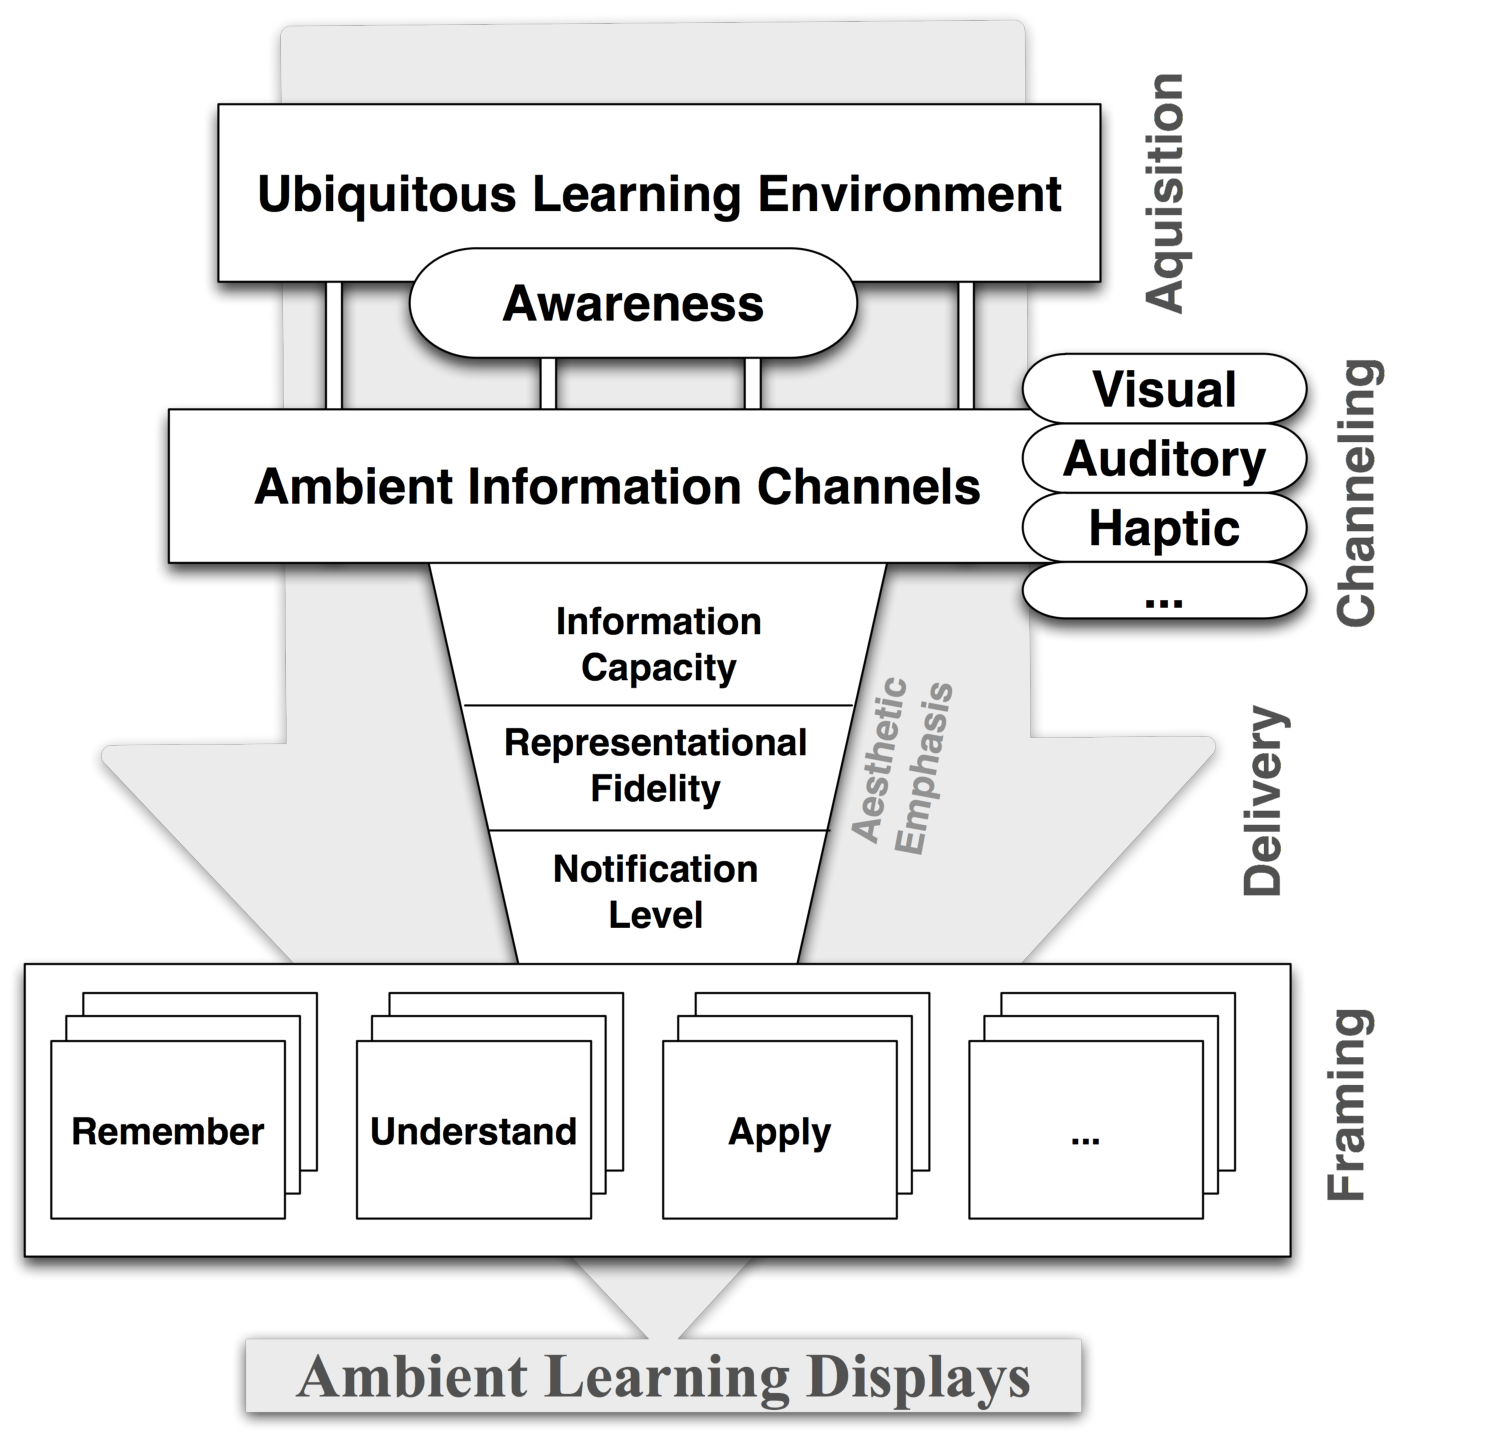
\includegraphics[width=0.9\textwidth]{figures/conceptual_framework}
\caption{Provisional conceptual framework for ambient learning displays} \label{fig:conceptual_framework}
\end{figure}

Within the framework awareness as one of the key concepts for informal learning support
\citep{Syvanen2005a} is used as acquisition instrument of the information relevant for
the learner within the ubiquitous learning environment \citep{Ogata2009b}. Consequently, the
acquired social, task, concept, workspace, knowledge, and context awareness information
sets up the conceptual framework. In order to present the acquired information in context
the ambient information channels model introduced by \citet{Specht2009} is utilised to carry
on the conceptual framework. Within the model ambient channels are used to deliver
information and services but also to feed information back into the system. Thereby,
information might be channelled into visual, auditory, haptic, odorous and respectively
tasting extraditable parts. To deliver the previously channelled information within the
ubiquitous learning environment ambient systems are used. Based on the comparison and
discussion of existing ambient information systems by \citet{Pousman2006b}, the
four design dimensions: information capacity, notification level, representational fidelity,
and aesthetic emphasis are used to design ambient systems as means of delivery. The
framing of the previously acquired, channelled, and delivered information in a learning
context then complements the conceptual framework. Based on the revised taxonomy of
educational objectives of \citet{Anderson2001} activities and objectives
enabled by the systems are matched to the types of knowledge and the cognition
processes involved. Thereby the taxonomy describes on the one hand several cognitive
process dimensions ranging from remembering over applying to creating and
distinguishes on the other factual, conceptual, procedural, and metacognitive knowledge.

But how would relevant information actually flow through the proposed conceptual
framework? Assuming an example setup where the users are asked to identify existing
learning objects/resources available in their proximity and match them according to the
context they are used in. Thereby context describes the relation of a learning scenario and
the location where the scenario takes place. This task addresses a simple cognitive
process dimension dealing with factual knowledge. An ambient system fed with
information reflecting the awareness needs of the users operating within the environment
would be used to support the task. Depending on the activity (derived from the addressed
cognitive process dimension) that needs to be supported, this information is channelled
through ambient information channels utilising different means and modalities to deliver
appropriate input for the ambient systems.

In such a setup creating workspace awareness could mean to use an ambient
visualisation method to describe possible learning scenarios. Concerning knowledge
awareness ambient audification methods could be used to create awareness when
someone enters the environment who created a certain learning object/resource and thus
might assist with the matching. And to provide a last example, vibration could be used as
a possible ambient haptification method to create context awareness reflecting the spatial
proximity of the learning object/resource to its learning scenario, respectively the
designated location.

\section{Research agenda}
Heading towards the implementation and manifestation of the envisioned ambient
learning displays an agenda for further research work has been set up incorporating the
outlined research questions and objectives. Based on this agenda the authors propose a
research project described in the following sections depicting an experimental design as
well as a usable evaluation technique.

In preparation of the research project a small-scale study \citep{Borner2010}\footnote{This publication is included as \textbf{Chapter 4} in this thesis.} has
already been conducted to gather opinion of experts in the field of mobile and ubiquitous
learning on the educational problem that can be solved by mobile learning. For this
purpose Concept Mapping \citep{Trochim1989} has been chosen as an appropriate method.
The method provides a structured approach to identify the experts� opinion on a given
domain, including both qualitative techniques and multivariate analysis approaches. The
result is a visual map of useful and important concepts that can then be used for further
elaborations. The study revealed that the two most important problem clusters are dealing
with �access to learning� and �contextual learning� aspects. Focusing on these problem
clusters and the covered problem descriptions in detail gives valuable insights on the
educational characteristics that define mobile and ubiquitous learning. For the presented
research agenda, these results of the study are used both as indicators for the educational
focus and as an instrument to validate the research findings.

The actual research design will begin with an extensive literature review covering in
general the aspects discussed in Section \ref{sec:ubiquitous_learning_characteristics} with a clear focus on ambient systems.
Regarding ambient systems there is a particular interest in existing applications used to
support personal, social, and environmental sense-making processes; derived patterns for
the design of such applications; and criteria and techniques that have been used for
evaluation. It is expected to find a large number of ambient systems that simply represent
information rather than supporting more complex cognitive processes. In any case, it
needs to be investigated if and how the applications are used within learning scenarios
and how they are evaluated on their effectiveness for learning.

Towards a profound conceptual framework that finally establishes the basis to build
prototypes for an experimental design, a lot of work has already been done as described
in Section \ref{sec:provisional_conceptual_framework}. Under the assumption that the information presented in context needs to
be acquired, channelled, delivered, and framed in the learning process, relevant research
findings, models, design dimensions, and taxonomies have been examined. Though the
outlined provisional conceptual framework for ambient learning systems is still subject of
modifications. Most probably the modifications will be due to the gathered insights from
the literature review of existing ambient systems for learning as well as the evaluation
techniques for respective applications.

\subsection{Experimental design}
Based on the prior literature review and the resulting conceptual framework analysis an
experimental design will be used to evaluate the prototypes built upon the conceptual
framework. Prior to the design it is planned to conduct formative studies to gather
insights on the specific usability needs and requirements of ambient systems and aid the
design process. Then a setup of ambient system prototypes, addressing specific cognitive
process dimensions, varied on the values of single design dimensions will be designed
and implemented. There is a particular interest in the effects on learning affected by the
way the ambient systems present information. The goal is to unveil in summative studies
how the single prototypes and prototype setups perform. The experimental design is
oriented on design-based research \citep{Baumgartner2003}, following a recurrent cycle
of designing an experiment, implementing the experiment, and evaluating the results in
order to review the experimental design again.

An example setup for such an experiment can be illustrated as follows: the ambient
system is fed with information reflecting the awareness needs of users operating within
the ubiquitous learning environment. Depending on the activity (derived from the
addressed cognitive process dimension) that needs to be supported, this information is
channelled through ambient information channels to deliver appropriate input for the
ambient systems. Each ambient design dimension can be varied on its distinguished
values. In this first experimental cycle the effect when manipulating these values on each
dimension will be measured, to figure out if and how this influences the performance of
the given activity and thus is effective for learning or not.

A possible hypothesis in such an experiment would be that ambient systems with a
low information capacity, an abstract representational fidelity, and a level of notification
that only makes aware, benefit the cognitive process dimension �remember�. To test this
hypothesis, the single ambient design dimensions would then be varied and compared to
each other. To do so, quantitative and qualitative data using data logs, questionnaires, as
well as a specific evaluation technique described in the next section will be collected.

\subsection{Evaluation technique} \label{sec:evaluation_technique}
To investigate and determine if the envisioned experimental prototypes are suitable to
support learners in authentic learning situations within ubiquitous learning environments
an appropriate evaluation technique is needed. Due to the nature of ubiquitous learning
finding suitable techniques is rather difficult. Users constantly move across contexts,
change environments, and usually are not restricted to act within a closed testbed for
evaluation. Thus, the experienced conditions cannot be controlled completely nor kept
similar. Therefore traditional evaluation techniques, such as pre-test/post-test designs, are
not sufficient. Instead the evaluation has to be done also in situ, taking into account the
current context, environment, and conditions the user is experiencing.
The challenge though is to find an appropriate technique that allows measuring the
effects in authentic learning situations. For ambient systems as well as ubiquitous
learning applications corresponding methods will be explored during the literature
review. One method that is already in the focus of attention is the experience sampling
method. The method has already been applied and examined for ubiquitous computing
applications. Derived from the field of psychology the technique is especially effective
for learning about situations and person-situation interactions and allows to �take place in
situ, involve several participants, take place over time, and collect both qualitative and
quantitative data� \citep{Consolvo2003a}. The technique uses several brief
adoptable questionnaires to let the participants report about their current activity and the
situation they are in. The participants are alerted in situ and asked to respond by filling
out a brief questionnaire. Traditionally used to evaluate aspects like emotion,
performance, or social interaction, the technique seems also sufficient to evaluate
ambient systems for learning.

Coming back to the example given in the previous section the method could be
applied as follows. Each participant is assigned to a specific task, which is to identify and
match existing objects/resources. To complete the task, the participants need to perform
certain actions. In the moment they completed the assigned task an event is triggered that
delivers an adapted questionnaire taking into account the current situation and context the
participant is in. The participants are then asked to indicate, for example which
information supported them to solve the task or which ambient system supported them to
solve the task. Using statistical methods on the surveyed qualitative and quantitative data
finally allows measuring the effectiveness of the ambient information presentation for
learning through the performance of the participants.

\subsection{Discussion}
While elaborating the research project some issues and challenges mainly related to the
undetermined target domain used to conduct the experiments, the evaluation of
ubiquitous scenarios in laboratory settings, as well as the importance of aesthetic design
for the experiments emerged. The issues related to the application domain are rather
complex. Quite reasonably the chosen application domain has a great influence on the
learning conditions. Authentic and situated learning usually occurs when learners are
strongly related to the placement they are active in and at the same time far away from
traditional (mostly formal) learning capabilities they would usually make use of. The
characteristics of the current placement and the requirements of the learners have in fact a
great influence on the assumptions the learners may have, the conditions they may find in
situ, as well as technical constrains of the settings. The chosen domain has an impact on
the conceptual framework and hence on the experimental design and the evaluation and
thus has to be chosen carefully.

The evaluation of ubiquitous scenarios in laboratory settings is self-contradictory.
While ubiquitous computing and the derived ubiquitous learning scenarios are
characterised by the �anywhere, anytime� paradigm, laboratory settings per se exclude
these features as they postulate the full control of all confounding variables. Evaluation
techniques need to take into account the current context, environment, and conditions the
user is experiencing within the situation that is observed. One possible solution has
already been mentioned in Section \ref{sec:evaluation_technique} describing a method already used to evaluate
ubiquitous computing applications \citep{Consolvo2003a}. Still, other available
methods need to be investigated and verified on their adequacy for the evaluation of
ubiquitous learning applications and thus ambient systems for learning.

Another issue is the importance and influence of an aesthetic design especially when
heading for an end-user product. The aesthetic emphasis is one of the dimensions
affecting the design of ambient systems \citep{Pousman2006b}. Within the
presented research project, this dimension will be mostly ignored. The reason for that is
mainly the focus on evaluating the effects of ambient information presentation on
learning and learning support rather than actually designing end-user products. In this
context emphasising the aesthetics design dimension of ambient systems too much is
simply not feasible for the research project, but definitely needs to be considered when
applying the outcomes to actual learning scenarios.

\section{Conclusions}
The chapter outlines the authors� vision of ambient learning displays � enabling
learners to view, access, and interact with contextualised digital content presented in an
ambient way. The vision is based on a detailed exploration of the characteristics of
ubiquitous learning and a deduction of informational, interactional, and instructional
aspects to focus on. Towards the vision essential research questions and objectives as
well as a conceptual framework that acquires, channels, and delivers the information
framed in the learning process are presented. Furthermore, a research agenda proposing a
research project is presented. This research project offers rich opportunities for the design
of environments following the mobile and ubiquitous learning paradigm, which gain in
importance for technology enhanced learning (TEL). Recently, the EU-funded project
STELLAR identified the grand research challenges for the future of TEL. As a guideline,
three themes have been formulated: connecting learners, orchestrating learning, as well
as contextualising virtual learning environments and instrumentalising learning contexts
\citep{STELLAR2009}. The authors� vision of ambient learning displays is strongly devoted
to the contextualisation theme; implicating manifold overlaps with the other themes.
Therefore the main research outcomes will also flow back into the contextualisation
theme. The main idea behind the theme is to encourage situated learning, while
supporting the learner�s mobility. Building on that, the key research questions in this
theme are:

\begin{compactitem}
  \item How can new forms of contextualised learning enable novel experiences for learners and for development of human competences?  
  \item How to support the mobility of the learner in distributed and multi environment learning settings, like the transition between real and virtual contexts?
  \item Which standards are needed to achieve interoperability and reusability of learning resources in this field? How to harmonise the existing learning standards?
\end{compactitem}

Comparing these key research questions with the presented vision, clarifies the relevance
within the field. The authors� vision of ambient learning displays highlights the
challenges and explores the possibilities that lie in the convergence of mobile and
ubiquitous learning in combination with the utilisation of contextualised digital content
as valuable resources to support learning.

Furthermore, the outlined research project delivers new scientific insights into the
authentic learning support in informal and non-formal learning situations. Within
ubiquitous learning environments the project will investigate if there is a measurable
benefit utilising ambient information presentation for a contextualised learning support.
From a practical point of view this research will flow into a framework that gives
guidelines for the future design of ambient systems for learning.
			\clearpage{\pagestyle{empty}\cleardoublepage}
	
	\addtocontents{toc}{\bigskip}
	\addtocontents{toc}{\bigskip}
	
	\part{Formative Studies}

		% To-Dos:

\chapter{Expert concept mapping study on mobile learning} % Write in your own chapter title

%\begin{quote}
%\textbf{*Abstract:} The present paper introduces concept mapping as a structured participative conceptualisation approach to identify clusters of ideas and opinions generated by experts within the domain of mobile learning. Utilising this approach, the paper aims to contribute to a definition of key domain characteristics by identifying the main educational concepts related to mobile learning. A short literature review points out the attempts to find a clear definition for mobile learning as well as the different perspectives taken. Based on this an explorative case study was conducted, focusing on the educational problems that underpin the expectations on mobile learning. Using the concept mapping approach the study identified these educational problems and the related domain concepts. The respective results were then analysed and discussed. The core educational concepts of mobile learning identified are: �access to learning�, �contextual learning�, �orchestrating learning across contexts�, �personalisation�, and �collaboration�. The paper is original as it uses a unique conceptualisation approach to work out the educational problems that can be addressed by mobile learning and thus contributes to a domain definition based on identified issues, featured concepts, and derived challenges. In contrast to existing approaches for defining mobile learning, the present approach relies completely on the expertise of domain experts.
%\end{quote}
\vfill
To inform the theoretical work as well as the design and development of ambient learning displays from different perspectives, several formative studies were conducted. This chapter describes an explorative study based on a concept mapping approach involving international experts from the field of mobile learning. These experts were asked to identify the major educational problems that can be addressed by mobile learning and cluster these problems into domain concepts that contribute to a definition of mobile learning. Although the study targeted on mobile learning, the results are in a broader view also valuable for the ubiquitous learning domain and thus for the research on ambient learning displays as they make use of key concepts, such as contextualisation and adaptation of information presentation to the user context and other situated factors.
\vspace{3em}

This chapter is published as: B�rner, D., Glahn, C., Stoyanov, S., Kalz, M., and Specht, M. (2010). Expert concept mapping study on mobile learning. \textit{Campus-Wide Information Systems}, 27(4), 240�253.

\clearpage

\section{Introduction}
So far there have been lots of attempts to define mobile learning, such as "learning that happens when the learner takes advantage of learning opportunities offered by mobile technologies" \citep{O'Malley2003}. The perspectives taken are either technocentric (like in the given example), consider the mobility of the learners, or rest upon the anytime/anywhere paradigm of existing content \citep{Winters2006,Taylor2006}. Each of these different perspectives is extensively discussed in the literature \citep{Sharples2007a,Traxler2009}, but by now there is no generally accepted definition, nor an agreement on which perspective to consider finding one. Especially the technocentric perspective is highly controversial as the underlying development of mobile technologies is continuously progressing, making the attempted definitions highly unstable \citep{Traxler2009}.

A more promising way towards a theory of mobile learning \citep{Sharples2005} seems to be the focus on the clarification of significant issues \citep{Sharples2007a}, research challenges \citep{ArnedilloSanchez2007}, case studies \citep{KukulskaHulme2007,Traxler2009}, or motivational or affective aspects \citep{Jones2006}. All these attempts contribute to a definition of key characteristics for mobile learning and sharpen the picture of what constitutes mobile learning rather then finding a precise definition. \cite{Traxler2009} even suggests replacing the question �what is mobile learning?� by the questions �what is learning in a mobile age?� or �what is mobile \textit{learning}?� focusing more on the educational part of the domain. Following this suggestion we decided to conduct an explorative case study \citep{Krathwohl,Yin1994} within the mobile learning domain that is not taking one of the perspectives mentioned earlier. Instead, the focus was set on the educational problems that underpin the expectations on mobile learning, while at the same time trying to find an adequate conceptualisation of these problems. Therefore the following research questions have been defined:

\begin{compactenum}
  \item What are the educational problems that mobile learning is trying to solve?
  \item Which problem clusters can be identified and how are they emphasised?
  \item How are the different problem areas related within the overall research domain of mobile learning?
\end{compactenum}

In the following sections we will introduce the applied method, analyse and evaluate the results, and finally discuss the findings and their relevance for the domain of mobile learning.

\section{Method}
To answer the formulated research questions, the presented study implements the concept mapping approach that has been initially described by \cite{Trochim1989,Trochim1989a}. This method has already been applied in several studies \citep{Stoyanov2004,Wopereis2005}. It provides a structured participative conceptualisation approach to identify clusters of ideas and opinions generated by experts for a given domain aspect. The collected data is then analysed via multidimensional scaling \citep{Kruskal,Davison1983} and hierarchical cluster analysis \citep{Anderberg1973,Everitt1980}. The result is a set of visual maps representing the generated idea and opinion statements as well as emerging statement clusters and thus important domain concepts. The method consists of several phases to prepare the collection of data and finally collect the data, each of which is described in the following sections.

\subsection{Preparation}
The initial phase of the method has three objectives: defining an initial focus or trigger statement for stimulating the generation of ideas and opinions,
selecting key dimensions for rating the generated statements, and selecting the participants.

Derived from the first research question the following trigger statement has been chosen: �The educational problem that mobile learning tries to solve
is��. Based on the experiences of previous studies \citep{Stoyanov2004,Wopereis2005}, �importance� and �feasibility� were selected as respective key dimensions. These qualitative dimensions emphasise different aspects of the practices within the domain. The importance dimension refers to the relevance of an educational problem within the mobile learning context. The feasibility dimension refers to the potential of mobile learning for contributing to a sufficient solution for the related educational problem.

Finally the participants were selected from the member list of the International Association for Mobile Learning \citep{IAMLearn2009}. In total 32 international
acknowledged domain experts have been invited to participate in the study. The invitees represented different stakeholder groups within the mobile learning domain, ranging from industry via research to educational practitioners. 20 out of the 32 invited experts accepted the invitation to participate in the study. Given to the international distribution of the participants, the communication as well as the data collection has been conducted entirely online via e-mail messages.

\subsection{Procedure}
The procedure to collect the data consisted of two phases: generation of idea and opinion statements and structuring the generated statements. Due to the characteristics of the method, the participants were actively involved in both phases of the data collection process. The phases are described in greater detail in the following sections.

\subsubsection{Generation of Statements}
In the first phase of data collection the participants were asked via e-mail to generate ideas and opinions on the previously defined trigger statement. The participants were instructed to simply reply to the e-mail message and include their identified educational problems as short bullet point statements underneath the trigger statement. The participants were free to generate as many statements as they wanted to. Although no direct control could be imposed on this process the participants were requested to describe exactly one educational problem in each statement and if possible limit the generation process to 10 minutes.

During this first phase, 11 experts generated 70 statements elaborating on the given focus in form of the trigger statement. Sighting the list of generated statements revealed an issue that needed to be solved before going on with the next phase. Almost each participant used an own structure to describe the ideas and opinions, which complicated the comparison of the statements. Therefore the statements were restructured into grammatically correct sentences and simultaneously revised for spelling mistakes. In doing so another issue was revealed, as some statements described more than one specific idea. To resolve the issue the relevant statements were taken apart and again restructured into grammatically correct sentences. Finally all the statements were compared to eliminate obvious duplicates, resulting in a list of 82 unique statements (e.g. �Maintaining continuity of learning across settings, such as between classrooms and museums on school field trips.�) that could be used for the next phase.

\subsubsection{Structuring of Statements}
In the second phase all participants were asked to structure the statements that were collected during the first phase. The participants were contacted no matter weather they generated statements in the first phase or not. The structuring of the statements involved two independent steps: grouping the statements based on their perceived similarity in meaning and the rating of the statements. In order to collect as much information as possible from the participants while reducing the communication overhead, the two steps were combined using a single e-mail message. To ease the process for the participants three documents were attached to each message. One provided the complete list of all unique statements. The other two documents were used to record the results of the grouping and rating. The participants were asked to perform the structuring of the statements within two weeks. 9 experts participated in the structuring phase, grouping and rating the statements that were previously generated.

Step A: Grouping

In the first step the participants were asked to group the statements based on their similarity in meaning. The participants were asked to copy the statements from one document containing all statements into a second document containing a prepared form with empty group containers. The participants were informed that they should place all statements into one group only, while each group should contain statements that were similar in meaning to each other. The instructions emphasised that the similarity must focus on the content of the statement and not on importance or feasibility of the statement. If a statement in the participants� opinion was unrelated to the other statements or stood alone as a unique idea, they were allowed to put this statement in its own group. In any case they were neither allowed to create arbitrary groups such as �misc� or �junk� groups. Again the experts were free to create as many groups as they liked, suggesting that in most cases using 10 to 20 groups should work out well. When finished the participants were asked to create a label for each group that described the included statements. In total, the experts created 111 groups with an average
of 12 groups per expert.

Step B: Rating

After grouping the statements the experts were asked to rate all statements in a third document. Each statement had to be rated on the key dimensions �importance� and �feasibility� on a 5-point Likert-scale. For importance the quantitative value 1 meant the statement described a less important educational problem that mobile learning is trying to solve and 5 meant the statement described a highly important educational problem. Respectively, for feasibility the quantitative value 1 meant solving the described educational problem through mobile learning is not feasible and 5 meant it is feasible to solve the problem through mobile learning.

\section{Results}
\subsection{Data Analysis}
To analyse the collected data the concept mapping approach proposes statistical data analysis techniques to map and then cluster the problem statements. Additionally the average ratings for each problem statement and the respective problem clusters are calculated and can be incorporated in the resulting visualisations for further interpretation. In the presented study all required calculations and visualisations for the analyses were accomplished using the spreadsheet application Microsoft� Excel� version 12.2.4 \citep{Microsoft2007} and the open source software environment for statistical computing R version 2.11.0 \citep{RDevelopmentCoreTeam2010}.

The concept mapping approach facilitates a non-metric multidimensional scaling analysis \citep{Trochim1989} to map the relation between the statements. In the present study, the statements were mapped onto a two-dimensional space, although multidimensional scaling can be applied across multiple dimensions. Trochim suggests the use of two dimensions, as the resulting bivariate distribution of points on the map is easier to visualise and interpret. Hence, the basis of the multidimensional scaling is a two-dimensional symmetric matrix of similarities of all problem statements. This matrix includes the correlations between the statements based on the expert grouping of the statements. For any two statements 1 is added to the respective intersection point within the matrix, whenever an expert placed the two statements in the same group. The result of the multidimensional scaling is a point map representing the Euclidian distance between the statements based on their similarity. Each point on the map represents a problem statement.

In order to group the statements on the map into clusters of statements, representing important domain concepts, the resulting point map is then used as input for a hierarchical clustering analysis, based on Ward�s algorithm for cluster analysis \citep{Trochim1989}. This technique isolates the conceptual relationships across statements as they are positioned on the point map obtained from the multidimensional scaling. The difficulty here is to identify a reasonable number of clusters. The concept mapping approach leaves this task open to the judgment and interpretation of the analyst.

Consequently for the presented study the optimal number of clusters was determined through minimising the cluster-size difference of the largest and the smallest cluster and maximising the size of the smallest cluster. After identifying the clusters they were manually labeled. The labels were derived from a list of group labels linked with the cluster and the statements within the cluster. Ideally the group labels provided by the experts converged towards a common domain concept represented by the cluster. If this was not the case, a keyword analysis at statement level was used to find a suitable label. The result of the hierarchical cluster analysis is a cluster map representing the emerging statement clusters and thus important domain concepts. In addition to the points of each problem statement, the map includes the convex hull of the problem clusters. This allows the analysis and interpretation of the relations between the single clusters as well as the associated statements.

\subsection{Problem Cluster Analysis}
As stated, the data analysis techniques were used to map the problem statements, identify, and label the problem clusters. The clusters represent the overarching domain concepts related to the educational problems addressed by mobile learning. Figure \ref{fig:cluster_map} shows the problem cluster map of the presented study.

\begin{figure}[!htb]
\centering
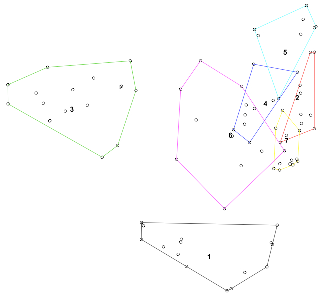
\includegraphics[width=0.75\textwidth]{figures/cluster_map}
\caption{Problem cluster map} \label{fig:cluster_map}
\end{figure}

The complete result data set including all problem clusters and statements can be found in Table \ref{tab:statement_rating}. The following 7 problem clusters covering 82 problem statements were identified:

\begin{compactenum}
	\item[(1)] Access to learning: The cluster covers 15 statements that are mainly related to the challenges of enabling learning in a mobile society. This includes educational problems that are related to flexible learning, including just-in-time learning, equal access to education and learning, and location-based learning. The cluster also covers remote learning and accessibility aspects.
	\item[(2)] Limitations for learning: 9 statements are included in the cluster. The statements cover challenges related to organisational and educational problems of educational institutions that result from different perceptions of the knowledge society in general and mobile technologies specifically among educators and learners. This also includes the problems of using of mobile technologies in formal learning scenarios.
	\item[(3)] Contextual learning: The cluster includes 18 statements that highlight the relation between learning and the context in which the learning takes place. The cluster covers individual aspects of situated learning, learning in context, and learning across contexts. Furthermore environmental aspects are included, such as making use of environmental affordances and a stronger interaction with the environment where the learning takes place.
	\item[(4)] Collaboration: 5 statements are included in the cluster. The statements cover challenges that are related to collaboration, sharing learning resources, and problems related to social interaction, such as difficulties of building a community during learning.
	\item[(5)] Personalisation: The cluster includes 8 statements. The statements range from educational problems with self-directed learning to mass-customisation of learning and reflect the potential of mobile learning to support personal learning processes and engage learners.
	\item[(6)] Orchestrating learning across contexts: 14 statements are included in the cluster, which deals with problems related to current educational practices. The cluster is strongly related to the contextual learning cluster, but focuses more on the organisational aspects that mobile learning can support.
	\item[(7)] Technology and technology adoption: The cluster covers 13 statements %. These statements address 
	addressing challenges related to the technological characteristics of mobile devices and factors of their adoption, including cost-effectiveness, usability, and user-acceptance.
\end{compactenum}

\begin{center}
\footnotesize
\begin{longtable}{l m{8.5cm} c c}
	
	\caption{Rating of problem clusters and statements}\label{tab:statement_rating} \\
 	\toprule
 	\multicolumn{2}{l}{\textit{Problem cluster}} & \multicolumn{2}{c}{\textit{Mean}} \\
 	\multicolumn{2}{l}{\ \textit{Statement}} & \textit{Importance} & \textit{Feasibility} \\
	\midrule
\endfirsthead
 	\multicolumn{2}{l}{\textit{Problem cluster}} & \multicolumn{2}{c}{\textit{Mean}} \\
	\multicolumn{2}{l}{\ \textit{Statement}} & \textit{Importance} & \textit{Feasibility} \\
	\midrule
\endhead
	\multicolumn{4}{r}{(continued)} \\
\endfoot

\endlastfoot

\multicolumn{2}{l}{1. Access to learning} & 4.03 & 3.59 \\
& 17. Access to learning resources and learning opportunities without the restrictions of location, time and cumbersome equipment or facilities & 4.44 & 4.00 \\
& 59. Access to information when and where it is required, through �just-in time� browsing of relevant information, and information push to support learning in context & 4.44 & 3.89 \\
& 41. Easing access to educational opportunities & 4.56 & 3.67 \\
& 25. Mobility of the learner & 4.00 & 4.11 \\
& 79. Including learners from rural areas & 4.22 & 3.89 \\
& 61. Accessibility of information in relevant everyday life and work situations & 4.33 & 3.67 \\
& 9. Learning at anytime & 3.89 & 4.00 \\
& 80. Developing third world countries� education & 4.11 & 3.78 \\
& 8. Learning from any location & 3.89 & 3.78 \\
& 11. Just-in-time information for immediate application & 4.11 & 3.56 \\
& 1. Limited access by some learners in remote locations & 3.67 & 3.89 \\
& 51. Enable learners in classroom settings to have equal access to rich resources and computational tools to support curriculum learning & 3.89 & 3.22 \\
& 78. Including learners with disabilities & 4.33 & 2.78 \\
& 4. Nomads who move from one location to the next while learning & 3.22 & 3.22 \\
& 45. Inequality of access to computers, learning resources and teachers & 3.33 & 2.44 \\
&&&\\
\multicolumn{2}{l}{3. Contextual learning} & 3.92 & 3.60 \\
& 53. Connect learning across contexts, including between formal and informal settings & 4.44 & 3.78 \\
& 16. Ability to discover and experiment in own context & 4.44 & 3.67 \\
& 30. The provision of access to knowledge in the context in which it is applied & 4.56 & 3.56 \\
& 33. Taking education out of classroom settings into meaningful settings & 4.00 & 3.89 \\
& 39. Interacting with your environment to achieve new knowledge from it & 4.22 & 3.67 \\
& 50. Under-utilisation of potentially rich learning resources in heritage sites, art collections and all sorts of other interesting places & 3.56 & 4.22 \\
& 73. Learning in context & 4.00 & 3.78 \\
& 74. Learning across contexts & 4.22 & 3.56 \\
& 58. Using technology to probe or to enrich understanding of the natural environment, and annotating the environment for the benefit of visitors & 3.67 & 4.11 \\
& 29. The design of augmented contexts for development problem to enable collaborative problem solving where learners generate their own �temporal context for development� & 3.89 & 3.78 \\
& 12. Learners cannot learn in context & 3.88 & 3.63 \\
& 57. Making use of affordances of locations to support learning & 3.88 & 3.63 \\
& 55. Enable enquiry-based learning in novel locations, through novel locations, and about  novel locations & 3.89 & 3.44 \\
& 63. Contextualisation of e-learning & 3.67 & 3.56 \\
& 56. Making use of space and environment as a backdrop for engaged spatial learning & 3.67 & 3.22 \\
& 70. The worthwhileness of location-based and contextual mobile learning & 3.56 & 3.33 \\
& 60. Enable learning through distributed conversation across contexts & 3.78 & 2.78 \\
& 3. Insufficient real life experience in the learning process & 3.22 & 3.22 \\
&&&\\
\multicolumn{2}{l}{6. Orchestrating learning across contexts} & 3.59 & 3.28 \\
& 20. Actively participate in learning activities outside of formal educational settings and facilities & 4.44 & 4.11 \\
& 24. Flexibility for the learner & 4.00 & 3.89 \\
& 54. Maintaining continuity of learning across settings, such as between classrooms and museums on school field trips & 4.11 & 3.67 \\
& 62. Documenting real time experiences of learners & 3.89 & 3.78 \\
& 37. Design suitable activities for the mobile learners & 3.89 & 3.67 \\
& 52. Orchestrate new forms of classroom pedagogy that require coordination of individual, small group and whole class activity & 4.00 & 3.33 \\
& 18. Provision of opportunities to contribute to the development/production of learning resources and course content without the restrictions of location, time and cumbersome equipment or facilities & 4.00 & 2.89 \\
& 47. Blinkered, old-fashioned views about education stopping when working lives begin & 3.44 & 3.22 \\
& 40. Anything is a potential learning scenario & 2.88 & 3.50 \\
& 28. Outside in, inside out problem, where cultural practices involving new digital media can be brought into formal learning institution, get enhanced inside the institution and in turn feedback into the digital world at large & 3.22 & 3.00 \\
& 46. Pressured, busy, fragmented, mobile lives leaving little quality time for conventional, place-and-time-dependent education & 3.33 & 2.89 \\
& 64. Transfer of training & 3.44 & 2.56 \\
& 49. Gaps (time lags) between traditionally scheduled learning sessions, limiting achievement, teamwork and collaboration & 3.11 & 2.56 \\
& 31. Refreshing the image and practice of institutional e-learning & 2.56 & 2.89 \\
&&&\\
\multicolumn{2}{l}{5. Personalisation} & 3.46 & 3.13 \\
& 81. Engagement of the learner & 4.44 & 3.56 \\
& 15. Not enough self-directed learning activities while learning & 3.67 & 3.78 \\
& 75. Self-directed learning & 3.89 & 3.11 \\
& 23. Finding new learning strategies that are suitable for the challenges of, and embraces the opportunities of, the knowledge and information age & 3.33 & 3.11 \\
& 43. Students exhibit passivity, boredom, indifference, low attention spans, and fail to complete their studies & 3.44 & 2.78 \\
& 42. The perception that there is a lack of student engagement & 3.11 & 2.89 \\
& 76. Learning with narratives & 2.89 & 3.11 \\
& 77. Mass-customised learning & 2.89 & 2.67 \\
&&&\\
\multicolumn{2}{l}{4. Collaboration} & 3.31 & 3.24 \\
& 19. Provision of opportunities to collaborate, share and publish learning resources and course content without the restrictions of location, time and cumbersome equipment or facilities & 4.33 & 3.33 \\
& 65. Spontaneous collaboration in situated learning & 3.67 & 3.33 \\
& 5. Lack of community building during learning & 3.11 & 3.33 \\
& 7. Not enough collaboration between learners & 2.89 & 3.44 \\
& 10. Learners not able to interact with experts from around the world & 2.56 & 2.78 \\
&&&\\
\multicolumn{2}{l}{7. Technology and technology adoption} & 3.32 & 3.05 \\
& 36. Make use of the affordable technologies that students have access to & 3.78 & 3.78 \\
& 66. Harness the fact that every student in every university owns a sophisticated communications device & 3.89 & 3.67 \\
& 21. Enhance teaching and learning within formal educational settings and facilities through handheld technologies & 3.78 & 3.44 \\
& 72. Get students to use their mobile devices constantly also in education & 3.67 & 3.56 \\
& 34. Helping educational institutions to offer learning aligned to the students� ownership, experience and use of technology & 3.89 & 2.89 \\
& 69. Dealing with small screens and difficult data input & 3.22 & 3.33 \\
& 32. Helping educational institutions understand the increasing and near universal ownership, acceptance and use of mobile devices across society & 3.22 & 3.11 \\
& 27. Cost-effectiveness for the providers of teaching and learning & 3.33 & 2.89 \\
& 26. Cost-effectiveness for the learner & 3.33 & 2.78 \\
& 71. Difficulties to reuse the products & 3.11 & 2.56 \\
& 38. Assess learning experiences to be accountable for the stakeholders & 2.78 & 2.67 \\
& 67. Revolutionise mobile learning, as the iPhone has revolutionised mobile telephony & 2.75 & 2.38 \\
& 68. Make mobile learning a revenue stream for telecommunication companies & 2.44 & 2.56 \\
&&&\\
\multicolumn{2}{l}{2. Limitations for learning} & 3.23 & 2.80 \\
& 22. Finding new teaching methodologies that are suitable for the challenges of, and embraces the opportunities of, the knowledge and information age & 3.44 & 3.22 \\
& 2. Lack of support to young learners, which have the mobile technology & 3.11 & 3.44 \\
& 14. Lack of ICT skills for the twenty-first century & 3.33 & 3.22 \\
& 82. Transformation of traditional education according to the needs of information society & 3.44 & 2.67 \\
& 48. Traditionally ineffective instruction and low learner performance in some subjects & 3.44 & 2.56 \\
& 6. Low motivation of learners who are mobile technology literate & 3.11 & 2.78 \\
& 13. Teachers not comfortable using mobile technology & 3.33 & 2.56 \\
& 44. Rigid assessment systems stifle creativity and innovation & 3.44 & 2.33 \\
& 35. Perceptions of technologically impoverished provision & 2.43 & 2.43 \\

\bottomrule
\end{longtable}
\end{center}

\subsection{Problem Emphasis Analysis}
A detailed analysis of the average rating of the problem statements indicates the experts� opinion about which statements refer to important and feasible educational problems related to mobile learning. Furthermore this analysis also allows estimating the importance and feasibility of the 7 problem clusters as domain concepts. The complete result data set including all problem clusters and statements with attached means can be found in Table \ref{tab:statement_rating}.

Starting with the problem statement emphasis, a statement was considered as important or feasible if the mean was at least 3.5 based on the 5 point Likert-scale rating. An average rating of 3.5 indicates that the experts rated the statement mostly as important or feasible. By taking both rating key dimensions into account the statements can be mapped into four quadrants. Figure \ref{fig:rating_map} shows the quadrants and the mapped statements without identifying the actual statements.

\begin{figure}[!htb]
\centering
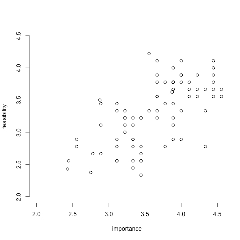
\includegraphics[width=0.9\textwidth]{figures/rating_map}
\caption{Statement rating map} \label{fig:rating_map}
\end{figure}

The first quadrant contains those statements that are relevant on both dimensions, with a high average rating on importance and feasibility. Thus included statements refer to the most relevant educational problems addressed by mobile learning. In the experts� opinion 34 statements are
located in this quadrant. The majority of the statements are related to the clusters �contextual learning� (13 statements), �access to learning� (11statements), and �orchestrating learning across contexts� (5 statements). The highest rated statements within these clusters are also included in the quadrant. The remaining statements are related to the clusters �technology and technology adoption� (3 statements) and �personalisation� (2 statements). The second quadrant contains statements with a high average rating on importance but low average rating on feasibility. The 13 statements in this quadrant can be considered to refer to important educational problems addressed by mobile learning, while sufficient solutions might go beyond the scope of mobile learning. The statements in this cluster are related to the clusters �contextual learning� (4 statements), �access to learning� (2 statements), �collaboration� (2 statements), �orchestrating learning across contexts� (2 statements), and �technology and technology adoption� (2 statements). The remaining statement is related to the �personalisation� cluster.

The third quadrant contains statements with low average ratings on both dimensions. 34 statements fall in this quadrant. These statements are considered to refer to educational problems that are not specifically related to mobile learning in the experts� opinion. The majority of statements in this quadrant are related to the clusters �limitations for learning� (9 statements) and �technology and technology adoption� (8 statements). The remaining statements are related to the clusters �orchestrating learning across contexts� (6 statements), �personalisation� (5 statements), �collaboration� (3 statements), �access to learning� (2 statements), and �contextual learning� (1 statement). The fourth quadrant contains statements with a high average rating on feasibility but low average rating on importance. The quadrant contains only a single statement that refers to a side educational problem to which mobile learning can offer solutions. This statement is related to the �orchestrating learning across contexts� cluster.

\begin{table}[!htb]
\centering
\caption{Highest emphasised problem statements}\label{tab:highest_emphasised}
\footnotesize
\begin{tabular}{m{9cm} c c}
\toprule
                  & \multicolumn{2}{c}{\textit{Mean}} \\
			\textit{Problem statement} & \textit{Importance}	& \textit{Feasibility} \\
\midrule
20. Actively participate in learning activities outside of formal educational settings and facilities. & 4,44 & 4,11 \\
17. Access to learning resources and learning opportunities without the restrictions of location, time and cumbersome equipment or facilities. & 4,44 & 4,00 \\
59. Access to information when and where it is required, through �just in time� browsing of relevant information, and information push to support learning in context. & 4,44 & 3,89 \\
41. Easing access to educational opportunities. & 4,56 & 3,67 \\
53. Connect learning across contexts, including between formal and informal settings. & 4,44 & 3,78 \\
16. Ability to discover and experiment in own context. & 4,44 & 3,67 \\
25. Mobility of the learner. & 4,00 & 4,11 \\
30. The provision of access to knowledge in the context in which it is applied. & 4,56 & 3,56 \\
79. Including learners from rural areas. & 4,22 & 3,89 \\
61. Accessibility of information in relevant everyday life and work situations. & 4,33 & 3,67 \\
\bottomrule
\end{tabular}
\end{table}

Concerning the importance and feasibility of the problem clusters, the average ratings of all problem statements included in a cluster needed to be considered. This analysis revealed that �access to learning� is rated as the most important cluster in the experts� opinion, followed by the clusters dealing with �contextual learning�, �orchestrating learning across contexts�, �personalisation�, �collaboration�, �technology and technology adoption�, and finally �limitations for learning�. Thus in the experts� opinion the accessibility and contextualisation of learning and education are the most important domain concepts that mobile learning can facilitate. The respective clusters also contain the majority of problem statements and as stated the highest rated statements, listed in Table \ref{tab:highest_emphasised}. Regarding the rated feasibility the emphasis is similar. The clusters of �contextual learning� and �access to learning� are rated as the most feasible domain concepts that mobile learning can facilitate, followed by the clusters dealing with �orchestrating learning across contexts�, �collaboration�, �personalisation�, �technology and technology adoption�, and finally �limitations for learning�.

\section{Discussion}
Based on the experts� emphasis the used concept mapping approach identified the most important educational problems that can be addressed by mobile learning. The identified problems are all related to the three main domain concepts �access to learning�, �contextual learning�, and
�orchestrating learning across contexts�, while most of them are related to the concept �access to learning�. This clearly reflects the claim on mobile learning to enable learning across context, facilitating and exploiting the mobility of the learners. The most emphasised issues mainly discuss learning activities and opportunities outside of formal settings, better contextualised and situated learning support, stronger connection between informal and formal settings, and the inclusion of rural and remote learners. Among others these issues indicate the most important current and future use cases for the implementation of mobile learning scenarios. On the other hand the experts considered issues related to technologies and their adoption and usage by teachers, learners and other stakeholders as less important to be addressed by mobile learning. The respective problems are mostly related to the domain concepts �technology and technology adoption� and �limitations for learning�. The emphasis given by the experts does also provide valuable recommendations. Educational institutes and organisations can draw direct conclusions about the core themes of future research agendas and implementation plans out of the study results. To provide an example, the most relevant problem statement within the �Contextual learning� cluster is �Connect learning across contexts, including between formal and informal settings.� The statement is positioned in the first quadrant of the statement rating map shown in Figure \ref{fig:rating_map}, as it got a high average rating on importance and feasibility. In the experts� opinion facilitating learning across contexts is one of the most important challenges in the domain of mobile learning. At the same time there seem to be sufficient solutions to cope with that challenge. The conclusion that can be drawn is that these solution need to be implemented on a short term.

Contrary to this example is the problem statement �Enable learning through distributed conversation across contexts.� covered in the same cluster. The statement is positioned in the second quadrant of the statement rating map with a high average rating on importance but low average rating on feasibility. So in the experts� opinion this challenge is also quite important, but it seems that there are no feasible solutions yet. Examining the statement clarifies this emphasis. To enable a distributed conversation across contexts is related to research in the field of e.g. computer supported cooperative learning. Even if the complex technology mainly coming from the field of mobile and ubiquitous computing is there, it still needs to be utilised in the learning context, which requires additional research efforts also within the field of mobile learning. In addition to the valuable emphasis, the approach also produced a problem cluster map representing the mobile learning domain concepts based on the similarity of the problem statements identified. The main concepts that characterise the educational challenges mobile learning has to cope with are �access to learning�, �contextual learning�, �orchestrating learning across contexts�, �personalisation�, and �collaboration�. The minor domain concepts are �technology and technology adoption� and �limitations for learning�. The produced map can also be used to relate the emerging problem clusters within the overall domain.

The map shows that the clusters �access to learning� and �contextual learning� appear to be independent domain concepts, as they are individually positioned beyond the centre. The other clusters seem to be more closely related and positioned near to the centre. The mapping shows that the �orchestrating learning across contexts� cluster is the central concept within the domain. This indicates that orchestration is the link between the different concepts within the domain of mobile learning. Both the �collaboration� and the �technology and technology adoption� cluster are positioned in close proximity to the central concept, illustrating that the covered problem statements need to be considered when dealing with orchestration and vice versa. The clusters of �personalisation� and �limitations for learning� are positioned a little bit further away from the central concept and thus do not need to be considered equally when orchestrating learning through mobile learning. The same applies for the distant clusters �access to learning� and �contextual learning�.

Focusing on the spatial extend of the single problem clusters, reveals that educational problems covered by the clusters �access to learning�, �contextual learning�, and �orchestrating learning across contexts� are in most cases only loosely related to each other. The mentioned clusters cover a wide problem space. In contrast the other clusters, especially �technology and technology adoption�, cover a relatively narrow problem space with closely related problem statements. On the one hand this underlines that the main domain concepts cover a diversity of educational problems and it might be useful to put more effort on a more finely granulated distinction in order to make further analyses easier to handle. On the other this fact shows that these concepts are still a major point of discussion and there is no agreement on a clear definition related to mobile learning.

\section{Conclusions}
The presented expert concept mapping study provides new insights on mobile learning and the educational problems that underpin the expectations on it. Especially the identified domain concepts contribute to the discussion about the key characteristics of mobile learning, while clarifying the major educational problems that can be addressed by mobile learning. Still the paper outlines only the major findings of the conducted study. The data collected as well as the results obtained from the concept mapping approach allow further profound analyses on single or multiple domain concepts or specific educational issues and their correlation to others. Furthermore the results can also be used to provide guidelines for upcoming discussions on the theoretical and technical developments within the domain of mobile learning. These aspects will be addressed in future work.
			\clearpage{\pagestyle{empty}\cleardoublepage}
	
	\addtocontents{toc}{\bigskip}
	\addtocontents{toc}{\bigskip}
	\addtocontents{toc}{\bigskip}
	
	\setcounter{footnote}{0}
	
	\chapter*{General Discussion\footnote{This Chapter incorporates discussions and conclusions from several publications.}\markboth{General Discussion}{}}
\addcontentsline{toc}{part}{General Discussion}
The research reported in this thesis aimed at identifying daily practices of adult lifelong learners and how they can be supported with technology in and across contexts. Therefore in a first step everyday patterns of lifelong learners were identified and mapped on a context model. From the perspective of the content, best practices to access educational resources from mobile devices were pinpointed as well as potential approaches to bind digital educational resources to physical spaces. Based on these findings, in a second step a set of prototypes to support lifelong learners were designed constituting a substantial base of tools and knowledge towards its evaluation in experimental settings. In a third step, these tools are evolved with the aim to facilitate lifelong learners to manage everyday life and learning activities in a more enjoyable and efficient way.
\section*{Main findings}
This research has concluded in the following achievements that are formulated together with future research challenges for ubiquitous support of lifelong learners with technology:

\subsection*{Understanding how lifelong learners learn using technology}
The results from the survey in \textbf{Chapter 1} shed light on different patterns describing how lifelong learners use their mobile devices to learn. Portable computers are perceived as the most commonly used device to learn. Participants owning a smartphone reported to be more constantly motivated to learn throughout the day (in contrast to feature-phone users. See figure \ref{survey_fig:2}), probably due to their perception of replacing "lost time� into perceived "productive time" when changing the context, commuting or in waiting times. Likewise, participants reported that they usually multitask while accomplishing learning activities with their mobile devices, especially  \em listening \em to content in which they reported to devote more time and in longer time slots. Regarding their preferred physical space to learn using mobile devices, there is an association between the learning activity being performed (i.e.  \em reading, listening, writing, watching \em ) and the concrete location where it takes place (i.e. living room, kitchen, bathroom. See figure \ref{survey_fig:5}). Additionally, the reports from the participants in the survey indicate that learning experiences are disrupted, whereas �finding a suitable time slot to learn during the day� is perceived as the most frequently found barrier.  

The findings concluded in this chapter are based on the reports from 147 participants from very specific contexts (three Dutch and Spanish universities, two high schools from Belgium and The Netherlands, two companies, one academy for skills-training). The questionnaire has ben released\footnote{Tabuenca, B. (2012) A Questionnaire for Lifelong Learners on Mobile Usage Habits, DSpace, Open Universiteit in the Netherlands, NELLL. Heerlen. Available online at  http:// hdl.handle.net/1820/4296} under open access so these results con be contrasted with further communities, contexts and countries. In coming research, we suggest to survey larger populations in subsequent iterations so these results can be documented and mapped to the ongoing evolution of the technology.

The results from the longitudinal study reported in \textbf{Chapter 9} conclude in the following time-patterns describing how lifelong learners learn throughout the day and the week. On the one hand side, students were able to log their study-time on personal mobile devices along the day with three different levels of intensity with regard to the number of time-logs performed (see figure \ref{fig:sload_10}): 1)  High Intensity. Time ranges between 9h to 15h and 18h to 22h. 2) Medium Intensity. Time ranges between 8h to 9h, 15h to 18h and 22h to 0h. 3) Low Intensity. Time ranges between 0h and 8h. On the other hand, findings show average time-logs per day fluctuate between 58 minutes to 83 minutes along the week (See table \ref{tbl:studyload_table5}). Students reported more minutes and more time-logs on Thursdays and Sunday. Longer time-logs were reported on Tuesdays and Wednesdays whereas the shorter ones are reported Mondays and Fridays.

Hereby lifelong learners explored how do they learn logging, tracking and monitoring one of the dimensions of context \citep{Specht2009}:  \em time \em . In further research, this tool represents a suitable approach for lifelong learners to track their learning habits while observing at the rest of the dimensions in their context (figure \ref{Esm_fig2}), namely, \em location \em (i.e. where do I learn?), \em relation \em (i.e. who with do I learn?), \em environment \em (i.e. which environmental circumstances affect me while learning?) and \em artefact identifier \em (i.e. which artefacts do I use to learn?).

\begin{figure}
     \centering
     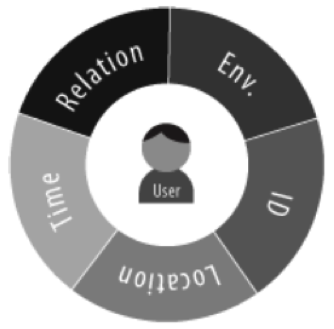
\includegraphics[width=0.4\linewidth]{img/Esm_fig2}
     \caption{Dimensions of mobile context \citep{Specht2009}}
     \label{Esm_fig2}
\end{figure}

\subsection*{Facilitate ubiquitous access to digital learning resources}
\textbf{Chapter 2} reviews the state-of-art of learning repositories featuring mobile access to digital resources. This review has concluded identifying different implementations to access content indexed by GPS coordinates, compass orientation, gesture recognition via accelerometer, radio frequency identification, infrared, visual code scanning, Bluetooth approximation, text-marker recognition or image recognition. Looking at the granularity of the resources, we found that easy to create and to consume contents on mobile devices, are those whose unit of construction is text, audio or video (minimum granularity). Going in depth to technical implementations, the conclusions of the review pinpoint to server architectures based on RESTful web-services featuring an Application Programming Interface (API), as well as HTML5 client, as suitable software implementations to facilitate content accessibility and scalability.  

Videos represent a big proportion of the learning materials provided in online courses. Most of the times, these videos are released in a LMS or shared in public repositories (i.e. YouTube, Vimeo). Watching a video requires the user to switch-on the device (x minutes), open a browser, login the platform, navigate to look for the desired resource (y clicks), and finally display the video on the mobile device (low resolution). This approach presents time, interaction and visualization barriers. In \textbf{Chapter 3}, we pilot the NFC-MediaPlayer, an ecology of resources comprising NFC tags, a multimedia casting tool and a learning content referratory, to cast videos from a mobile device to an HDMI display interpreting the commands (i.e. play, pause, forward, cast) of the NFC tag that is tapped with the mobile device. This novel ecology facilitates seamless access to video contents reducing the time to start the learning activity, reducing the number of clicks to access the learning content (to zero clicks), and casting in High-Definition quality, learning contents that are normally casted in small-sized screens on mobiles, tablets or laptops. Additionally, we share the �know how� releasing the source code under open license to foster its scalability to other applications and communities.

Findings reported in chapter 2 show different channels to enable ubiquitous access to digital learning resources stored in content repositories using mobile devices. The scalability of new mobile clients providing access to content stored in repositories is highly dependant on the existence of an API, as well as the granularity of the content which is served. Hence, we conclude that learning contents offered with a low granularity (i.e. text, video, audio) and repositories implementing RESTFul web-services facilitate access to digital resources to mobile app developers, smartphone users and consequently to a broader range of lifelong learners.

\subsection*{Linking learning activities with everyday life activities and the physical world objects}
\textbf{Chapter 2} identified NFC technology as a prominent trend in the field of mobile technology in the last years. This technology is particularly relevant for lifelong learners due to its reduced complexity to accomplish predefined actions (zero-clicks) and facilitating a smooth integration of learning activities into physical spaces. \textbf{Chapter 3} reviewed scientific literature in which NFC has been used with learning purposes and potential uses for learners are classified. As a consequence of this review,  \em activity recognition \em and  \em life logging \em are highlighted as relevant fields to link learning activities with everyday life activities. Indeed, lifelong learners' activities are scattered along the day and in different locations making difficult to manage learning goals and to have an account of how much time is devoted to each one of them. Nevertheless, the results reported in \textbf{Chapter 1} show that lifelong learners frequently recur to preferred learning environments throughout their learning journey (physical spaces, devices, or moments). Sometimes the physical environment itself may relate to learning activities in other cases only temporal patterns might be of relevance while the physical location is not crucial. Therefore, this research has provided cues for lifelong learners to introspect their autobiography as learners, to identify successful learning environments, to bind them to self-defined learning goals, to keep track of the time devoted to each goal, to monitor their progress, and consequently to understand how does he/she learn. The NFC-LearnTracker presented in \textbf{Chapter 6} supports lifelong learners in those functions, providing a suitable tool to foster awareness on preferred learning environments, to manage learning goals, to have an accurate account on time devoted to learn, and to analyze personal learning patterns.

The NFC-LearnTracker (released under open source), and the empirical studies identified in Chapter 3 imply an important base of knowledge to scaffold potential scenarios linking learning activities with everyday life objects using NFC technology.  \cite{Livingstone2007} analysis on work-time and learning activities stresses the lack of longitudinal studies in job-related informal learning. In further research, the NFC-LearnTracker and its support to learning processes should be evaluated in real scenarios in which learners use their own NFC-enabled smartphones in longitudinal studies. This tool might be useful to determine whether there is a positive or negative correlation between the duration of the learning moments and the performance learning.

\subsection*{Awareness of available resources in everyday life}
This thesis has shown different cues to foster awareness on available resources, locations and moments to learn in everyday life using technology. In \textbf{Chapter 4} we proposed sampling of learning experiences on mobile devices as key benchmarks for lifelong learners to become aware on which learning task suits in which context, to set realistic goals and to set aside time to learn on a regular basis. A classification framework for sampling of experiences on mobile devices has been presented as an approach to explore variations to deliver, dispatch and answer notifications in context. These framework is not only useful when prompting notifications to second persons (e.g. from teacher to student), they are significantly more powerful and accurate when they are self-reports due to the fact that the lifelong learner has an intrinsic motivation to know himself as a learner and consequently to provide truthful reports having only himself as a reference. This classifications framework is instantiated along the thesis for the prototypes presented in \textbf{chapters 4, 6, 8 and 9}.

This self-reporting technique represents an interesting approach for lifelong learners to get actively involved in knowing their own learning day. The ESM instantiated in personal mobile devices is very suited for lifelong learners to explore their own specific context, learning style, and available resources to model each learning moment.

\subsection*{Develop artefacts to support lifelong learners}
This thesis has resulted in the development of different artefacts and software prototypes that facilitate the implementation of educational designs as well as support the connection of informal learning experiences with formal learning activities in and across contexts. This research comprises the development of six different software tools shared in open source, namely, NFC-MediaPlayer ( \textbf{Chapter 3} ), ESM app ( \textbf{Chapter 4} ), Mobile Authoring Tool for ARLearn ( \textbf{Chapter 5} ), NFC-LearnTracker ( \textbf{Chapter 6} ), smart ecology of resources for effective time management ( \textbf{Chapter 7} ), and the LearnTracker framework ( \textbf{Chapter 9} ). 

The set of tools presented in this research facilitate connecting informal and formal learning experiences featuring author of learning resources in authentic scenarios, tracking and monitoring time devoted to learn across contexts, and providing seamless access to learning resources in frequently used lifelong learning scenarios. All these tools are released under open source\footnote{Source code repository of tools piloted in this thesis: https://code.google.com/p/lifelong-learning-hub/source/clones} and might be adapted or extended in further research.

\subsection*{Identify barriers for digital competence in lifelong learners}
This thesis has demonstrated that the combined use of multiple devices might lead to important differences in digital competence from one learner to another. Findings from \textbf{Chapter 8} pinpoint to differences with regard to \em familiarity with the mobile device \em , \em familiarity with the operating system of the device \em and \em the complexity of the user interface \em  as key aspects to take into account when designing technology to support lifelong learners. Likewise, the results obtained in \textbf{Chapter 9} show that the \em usability of the tool \em , the \em number of clicks \em to accomplish an action, and the \em response time \em , are key aspects to take into account in the design of tools to support lifelong leaners in long term.

\subsection*{Foster reflective practice on meta-learning}
All along this thesis we have explored the effectiveness of mobile notifications to foster reflection on meta-learning. In a first step ( \textbf{Chapter 4} ) we explored the variables affecting the user when sampling experiences on mobile devices and the ESM apps was developed to identify user preferences with regard to the way to receive, dispatch and answer notifications on mobile devices. The results of the pilot evaluation show that learners preferred to receive notifications \em on-demand \em rather than \em time-scheduled \em or \em random basis \em.  Additionally, they preferred prompt notifications as well as answer notifications in \em text \em format, in contrast to \em audio \em , \em picture \em or \em audio \em formats.

In the two studies presented in \textbf{Chapter 8}, we used reflection amplifiers \citep{Verpoorten2012} instantiated with mobile notifications to make what users learn, a deliberate object of attention. Findings in the first experiment show that (secondary school) students do not have a habit to see themselves as learners and to develop a professional awareness about their daily activity at work/school. In the second experiment we researched variations in the �timing�, �frequency�, and �complexity� of notifications fostering reflective practice on learning, and its impact on "knowledge" and "motivation". Findings in this experiment show better "knowledge" scores for the group of learners that were assigned with the least complex interactions on mobile devices during the reflection exercise. 

Based on the lessons learned from these experiences, the longitudinal study described in \textbf{Chapter 9} evolved the NFC-LearnTracker presented in \textbf{Chapter 6}, to observe variations in the �timing� and �content� of the notifications. Findings reveal positive effects of tracking learning time in �time-management� skills. These results not only provide evidence of the benefits of recording learning time, but also suggest relevant cues on how mobile notifications should be designed and prompted towards self-regulated learning.

\subsection*{Self-defined internal feedback}
The differentiation among external and internal feedback is crucial if one investigates the effects of feedback as a self-regulated learning process \citep{Narciss2007}. Hence, the last phase of the research shifts the perspective from externally designed notifications (designed by the teacher, instructional designer or researcher) to self-designed notifications (designed by the learner) evolving the NFC-LearnTracker to an ecology of resources in which lifelong learners can design notifications served via an ambient learning display \citep{Borner2013}, and map them to events happening along the learning process. This ecology lets the user configure which signal fits better each one of the given events (see Table \ref{tbl:nfceco_table1}).

In further research this tool might support to investigate the impact in self-regulated learning of externally designed notifications (external feedback) in contrast to self-defined notifications (internal feedback).

\section*{Limitations of this research}
By identifying daily practices from lifelong learners this thesis has contributed towards a common understanding of how lifelong learners learn to support them with ubiquitous technology. However, several factors limited the conducted research:

Regarding \em understanding how lifelong learners learn using technology\em , the results reported in chapter 1 are based on personal perceptions. Concepts like \em motivation to learn \em or \em learning intensity \em might be understood differently depending on the user that is answering the questionnaire. Additionally, the time patterns found in chapter 9 might be influenced by the assignments scheduled by the teachers for this specific course. There is a need to extend this research to larger groups from several disciplines to obtain a more accurate vision on how lifelong learners learn (throughout the day and along the week) independently on the courses they are enrolled.

Regarding \em facilitating ubiquitous access to digital learning resources\em , the results presented in chapter 2 and 3 show different shortcuts facilitating access to content stored in repositories. Nevertheless, most of the technologies presented in these reviews were piloted in special settings (i.e. lab experiments, restricted scenarios, augmented reality) that might be not extrapolated to real case scenarios. 

Regarding \em linking learning activities with everyday life activities and the physical world objects\em , the evaluation of the NFC-LearnTracker has been performed in an artificial context (technology enhanced learning workshop). This tool should be tested in longitudinal studies with personal mobile devices and in lifelong learning settings. A realistic scenario must contemplate that the single decision to start using the tool should be triggered by an intrinsic motivation from the user to explore own learning patterns rather than an externally imposed tool. The effects in self-regulated learning should be explored in further research.

Regarding \em awareness of available resources in everyday life\em , the pilot presented in chapter 4 has raised the following limitations: first, this pilot was tested in an exceptional learning context. Real lifelong learning scenarios imply daily routines like workplaces, transitions, etc.; second, the duration of the experiment was too short. Modelling one�s lifelong learning day implies a long-term experiment in which moments of the day and moments of the week are explored. 

Regarding the \em development of artefacts to support lifelong learners\em , we have released several prototypes that might need adaptations depending on the contingencies of the context in which they are evaluated, and the version of the operating system in which they are deployed. Most of the artefacts presented in this thesis were developed for Android devices. These tools might need to be extended to other operating systems in further research.

Regarding \em foster reflective practice on meta-learning\em , the experiment presented in chapter 4 involved 12 voluntary researchers in the field of Technology Enhanced Learning (TEL). The small-scale of the participation, the short duration of the experiment, and the fact the participants had an expertise in TEL might have biased the reported results. These results should be contrasted with further larger studies.

Most of the conclusions reported in Chapter 9 are based on the recordings from 13 students taking part in an online university course during 4 months. Findings reported in this thesis might need to be contrasted with larger groups. Some of the effects identified in the intermediate measures of Chapter 9 might be moderated as a consequence of sequencing effects, and not only caused by the treatment delivered during that specific treatment. More research is needed providing these treatments to independent groups.

Hence, Lifelong learners model daily learning routines based on intrinsic motivations and personal decisions taken in real circumstances. The tools used in these studies were not discovered by the learners themselves, but rather offered to them from external researchers. Thus, initiatives to mentally evoke what they have learned throughout the day to turn the learning experience into a deliberate object of attention and reflection are more powerful when they come from personal inquietudes rather than from external invitations.

Most of the work reviewed in this thesis is limited to scientific literature. Nevertheless, a big proportion of the developments from lifelong learners are not documented because they are based on personal understandings and consequently do not have a relevant scientific value.

		\clearpage{\pagestyle{empty}\cleardoublepage}
	
\backmatter
	
	% Acknowledgements

% To-Dos:
%
% Footnote
% Figures
% Tables
% References

\chapter*{Acknowledgements\markboth{Acknowledgements}{}} % Write in your own chapter title
\addcontentsline{toc}{chapter}{Acknowledgements}

For their continuous support I would like to thank my family and friends, especially my girlfriend, Jessica Biermann, for allowing me to start this journey and supporting me to finish it, as well as my parents, Marlene B�rner and Hans-Joachim Sternkopf, for making everything possible.

Furthermore, I would like to thank my colleagues and all the people I met while conducting this research for their inspiration, review, and support of my work. Special thanks to my \textit{promotor} Marcus Specht and my \textit{co-promotor} Marco Kalz for their outstanding supervision and guidance as well as to Mieke Haemers for her organisational wisdom.

Last but not least, I would like to thank my \textit{paranimfen}, \mbox{Halszka} \mbox{Jarodzka} and \mbox{Bernardo} \mbox{Tabuenca}, for their broad support and friendship, my \textit{promovendus} companion, \mbox{Sebastian} \mbox{Kelle}, for his advice and the mutual cultural exchange, as well as the band Tocotronic for their creative and inspiring song titles.

\section*{Funding sources}
The research project presented in this thesis was mainly funded by the STELLAR Network of Excellence, the OpenScout project, and the weSPOT project. STELLAR is a 7th Framework Programme project funded by the European Commission, grant agreement number: 231913 (http://www.stellarnet.eu). OpenScout is a 7th Framework Programme eContent+ project funded by the European Commission, grant agreement number: 428016 (http://www.openscout.net). weSPOT is a 7th Framework Programme research project funded by the European Commission, grant agreement number: 318499 (http://wespot-project.eu).

The projects reported in \textbf{Chapter 5} and \textbf{6} have been partially funded by a SURFnet innovation grant for sustainable ICT solutions and partially by the Centre for Learning Sciences and Technologies (CELSTEC) of the Open Universiteit in the Netherlands.

As part of a subordinated small-scale study on location-based and contextual mobile learning, the study presented in \textbf{Chapter 4} was conducted in cooperation with the Learning Sciences Research Institute (University of Nottingham) within the framework of the STELLAR Network of Excellence.

The study presented in \textbf{Chapter 7} was conducted in the context of two lectures. Special thanks to all participants of the SIKS advanced course on �Technology-Enhanced Learning� and the master students attending the guest lecture on �Ambient Learning Displays� as part of the RWTH master course on �Advanced Learning Technologies�.

Finally the study presented in \textbf{Chapter 10} was partly funded by the European Regional Development Fund (ERDF), regions of the Euregio Meuse-Rhine (EMR), and the participating institutions within the implementation and research project �EMuRgency - New approaches for resuscitation support and training� (EMR.INT4-1.2.-2011-04/070, http://www.emurgency.eu) under the INTERREG IVa programme.
		\clearpage{\pagestyle{empty}\cleardoublepage}

	\bibliographystyle{apalike} % THIS sets the bibliography style. requires natbib in the header file.
	\renewcommand{\bibname}{References}
	\addcontentsline{toc}{chapter}{References}
	\bibliography{bibtex/Ambient_Learning_Displays.bib} %.. and this makes the actual bibliography appear after the list of figures and before the appendix.
	
	\addtocontents{toc}{\bigskip}
	\clearpage{\pagestyle{empty}\cleardoublepage}
	
	\setcounter{footnote}{0}
	\chapter*{Summary\footnote{This chapter incorporates abstracts, discussions, and conclusions from several publications.}\markboth{Summary}{}}
\addcontentsline{toc}{chapter}{Summary}

Lifelong learners learn in scattered moments throughout the day and the week, and they have to balance learning activities with work, family and leisure activities. In this thesis, we have explored how, when, what and where lifelong learners are learning by using their mobile devices as a key channel to support them across contexts. 
The research conducted for this thesis has been guided by the following objectives:

\begin{enumerate}
\item Understanding personal learning ecologies of lifelong learners.
\item Facilitate ubiquitous access to digital learning resources.
\item Link learning activities with everyday life activities and the physical world objects.
\item Develop artifacts and software prototypes that allow the implementation of educational designs in which the learners connect informal learning experiences with formal learning activities in and across contexts.
\item Identify barriers for digital competence in lifelong learners. 
\item Foster reflective practice on meta-learning. 
\end{enumerate}

In this thesis, smartphones support lifelong learners across contexts (e.g. at home, at work, commuting, having a break) since they are always carried around with the learner. \textbf{Chapter 1} identifies learning patterns in daily life environments as a starting point to understand how lifelong learners learn using their mobile devices, and in which contexts they might need support. 

Offering educational resources openly is one of the key policies to facilitate universal access for lifelong learners. In \textbf{chapter 2} we have observed the current support from content repositories to mobile devices, identifying best practices and suitable architectures for the implementation of software that might facilitate universal access to content stored in repositories. Additionally, smartphones enable learners to author educational resources not only providing channels to share, remix or re-contextualize these, but also capturing the context in-situ and in-time. As a further matter, authoring educational resources in a mobile context is an authentic experience where authors can create learning resources inspired on their own daily life activities and reflections. 

A strength of lifelong learners is their motivation to learn and their continuous career development. Hence, they continuously try to understand and improve the way they learn identifying best contexts (i.e. time, location, technology) and embedding learning activities into daily life activity. In this thesis, we offered lifelong learners to introspect their learning habits, and annotate their reflections on personal mobile devices as key benchmarks to become aware of successful learning environments and to identify their learning preferences in context (i.e. preferred time, location, resources). A classification framework for sampling of experiences on mobile devices is presented (See figure \ref{fig:Esm_fig1}) and instantiated in \textbf{chapter 4}. Later on, this framework is again evaluated in experimental settings (\textbf{chapters 6, 8, 9}). 

In \textbf{chapter 6} we identify the lack of support for learning activities across locations, devices, and environments, as well as, the necessity to link learning activities with everyday life activities as key challenges for lifelong learners. There is very little research on how to link the different everyday contexts of lifelong learners and their learning activities in these different settings. As reported in \textbf{chapter 1}, lifelong learners recur to certain physical spaces (e.g. sofa, desktop) or moments (e.g. commercial breaks on TV, waiting times, commuting) to accomplish their learning activities. The NFC-LearnTracker presented in this thesis was recognized as a relevant tool with the potential identify those successful learning environments, to manage self-defined learning goals, to keep track of the time devoted to each learning goal, and to monitor their progress with learning analytics visualizations.

In this thesis we aimed at supporting learners to understand the way they can better learn using technology.  We focused on two specific key competences for lifelong learning \citep{EuropeanCommission2007}, namely, �learning to learn� and �digital competence�.

On the one hand side, �learning to learn� implies the learner to understand how to make the best use of own skills and available resources towards the accomplishment of self-defined learning goals. Therefore, in \textbf{chapter 8} we instantiate again the classification framework for sampling experiences (figure \ref{fig:Esm_fig1}) by prompting learners compact and structured notifications suggesting to examine and evaluate their own learning. These notifications were prompted as structured and repeated introspective episodes, offered during the course of the learning action as well as after the learning action, to make learning visible. The results show that students do not have a habit to see themselves as learners and to develop a "professional" awareness about their daily activity at work/school. The effectiveness of mobile notifications to foster reflective practice on meta-learning is further researched in the longitudinal study reported in \textbf{chapter 9}. In this study we analysed the timing and the content of the notifications. The findings conclude that notifications pushed at fixed times of the day moderate positively the measure of time management. These results are consistent with the answers reported by the learners regarding their timing preference in which, notifications at 10h were preferred over notifications at 20h as well as over notifications randomized in time. Another reason to argue on these results might be that students prefer notifications that persuade them to (pre-)�plan ahead� their learning day, rather than (post-)�look backward� their learning day or (in-action) �plan� at any moment of the day. Observing at the content of the notifications, the findings in the experiment suggest that notifications containing learning analytics and tips for self-regulation influence positively the skill of time management. More specifically, notifications containing learning analytics resulted in slightly higher scores. Likewise, \textbf{chapter 9} provides an interesting perspective on how learners devote their time to learn throughout the day, along the week and in long term.

On the other hand, �digital competence� involves the confident and critical use of technology to learn, work, and communicate in personal and social life. Nowadays, technology is constantly shaping the way we learn, thus designing interfaces that are easy to use and to integrate into daily life activity becomes increasingly relevant for lifelong learners. This assumption is reinforced by the results reported in the second study from \textbf{chapter 8}, in which the group assigned with the least complex interactions on mobile devices achieved higher knowledge and motivation scores.

The results from the survey in \textbf{chapter 1} show that lifelong learners reported their living room (and sitting in the sofa) as the most suitable environment to watch videos using their mobile devices for learning purposes. In \textbf{chapter 3}, we orchestrate an ecology of digital resources in the context of this specific environment to facilitate casting of video content stored in the cloud by lowering the complexity of interactions with devices (i.e. reducing the time to start the learning activity, reducing the number of clicks to access the learning content), as well as improving the resolution casting HD quality as an alternative to small-sized definition on mobiles, tablet or laptops. 

In this research, we investigated different ways to foster the competence of �learning to learn�, using SMSs and mobile chart visualizations as channels to provide guidance (external feedback). The differentiation among external and internal feedback is crucial if one investigates the effects of feedback viewing the process of knowledge acquisition as a self-regulated learning process \citep{Narciss2007}. Hence, in the last stage of the research (\textbf{chapter 7}) we extended the NFC-LearnTracker implementing a ecology of resources for lifelong learners to customize their internal feedback based on own occasional learning priorities and contingencies.


		\clearpage{\pagestyle{empty}\cleardoublepage}
	
	\setcounter{footnote}{0}
	% To-Dos:
%

\chapter*{Samenvatting\footnote{Dit hoofdstuk bevat samenvattingen van, discussies over en conclusies uit verschillende publicaties.}\markboth{Samenvatting}{}}
\addcontentsline{toc}{chapter}{Samenvatting}

%\vfill
%\clearpage

In dit proefschrift worden de resultaten gepresenteerd van het uitgevoerde onderzoek en de ontwikkeling van ambient learning displays. De resultaten worden in drie delen gerapporteerd: theoretische grondslagen, formatieve studies en empirische bevindingen. Een uitgewerkt conceptueel kader en een uitgebreid literatuuronderzoek werden gebruikt om het veldonderzoek te verkennen en deze vormden de basis voor verder onderzoek. \textbf{Hoofdstuk 1} schetst de visie op ambient learning displays - het voor leerlingen mogelijk maken om gecontextualiseerd digitale content die op een ambiente manier aangeboden wordt, te bekijken, zich toegang ertoe te verschaffen en ermee te interageren. Deze visie is gebaseerd op een gedetailleerde verkenning van de kenmerken van ubiquitous learning en een gevolgtrekking van informatieve, interactionele en educatieve aspecten waar we ons op richten. Om te zorgen voor een theoretische grondslag voor het volgende onderzoek, werden relevante onderzoeksresultaten, modellen, ontwerpdimensies en taxonomie�n onderzocht. Het resultaat was een conceptueel kader dat ambient learning displays omschrijft. Het kader bestaat uit delen die zich toelegden op de gebruiker en op context data-acquisitie, op het kanaliseren van informatie en op het doorgeven van gecontextualiseerde informatie, ingekaderd in een leerproces. 

Het eerste deel van de uitgevoerde literatuurstudie, gepresenteerd in \textbf{Hoofdstuk 2}, toont kenmerken en geclassificeerde prototypische ontwerpen en belicht het daadwerkelijke gebruik van de beschreven ambient displays, de context waarin ze toepasbaar zijn en de aangesproken domeinen alsook het type van uitgevoerde studies, met inbegrip van de gebruikte methoden en evaluatiebenaderingen om hun doeltreffendheid en het effect te meten. De resultaten toonden aan dat het verkrijgen en het doorgeven van informatie via ambient displays in lijn was met het gepresenteerde conceptuele kader. De middelen om de informatie en het inkaderen in een leerproces te kanaliseren behoeven verder onderzoek. Het literatuuronderzoek werd voortgezet in \textbf{Hoofdstuk 3}. Dit tweede deel was gericht op het werkelijke gebruik van ambient displays in een leeromgeving. Het doel was om ambient displays te beoordelen met een expliciet of impliciet leerdoel en het indelen van de respectievelijke prototypes op grond van een uitgebreid classificatiekader met informatieve en interactionele vormgeving van de prototypes, onderzoeksdoelstellingen en resultaten van de gerapporteerde empirische studies, evenals afleidbare educatieve eigenschappen. Uit de resultaten bleek dat het expliciete gebruik van ambient displays voor leeractiviteiten geen prominent onderzoeksonderwerp was, terwijl ambient displays impliciet al werden gebruikt ter ondersteuning van leeractiviteiten ter stimulering van situationeel bewustzijn door het benutten van feedback. Het vergelijken van de overeenkomende prototypes met het ingevoerde classificatiekader heeft geleid tot de eerste algemene gevolgtrekking met betrekking tot het ontwerp, rekening houdend met educatieve kenmerken.

Verschillende formatieve studies vormden input voor het theoretische werk, alsmede voor het ontwerp en de ontwikkeling vanuit verschillende perspectieven. \textbf{Hoofdstuk 4} beschrijft een exploratieve studie die werd uitgevoerd om input te geven aan het onderzoek van ambient learning displays. Door domeinexperts te vragen naar de gebruikte aanpak voor concept mapping werden de voornaamste educatieve problemen ge�dentificeerd, welke door mobile learning opgelost kunnen worden en daarna werden deze problemen gebundeld in domeinconcepten die bijdragen aan een definitie van mobile learning. De belangrijkste domeinconcepten die werden ge�dentificeerd, waren "access to learning" en "contextual learning". Deze reflecteerden de potentie om het mogelijk te maken om contextoverstijgend te leren met behulp van mobile learning en het vergemakkelijken en het benutten van de mobiliteit van lerenden. Hoewel de studie was gericht op het domein van mobile learning, werden de resultaten in een breder perspectief ook waardevol geacht voor een ubiquitous learning omgeving en daarmee voor het verrichte onderzoek. 

De resultaten van twee projecten, die input gaven aan het ontwerp en de ontwikkeling van ambient learning displays, werden gepresenteerd. Het eerste project, gepresenteerd in \textbf{Hoofdstuk 5}, onderzocht en ontwikkelde een infrastructuur die energiebesparing ondersteunt op de werkplek. Het doel was gegevens over het energieverbruik zichtbaar en toegankelijk te maken voor de medewerkers door middel van het verschaffen van dynamische feedback in situ over het verbruik. De gepresenteerde resultaten toonden de algemene interesse in het onderwerp en gaven de effectiviteit aan van de ge�ntroduceerde middelen met betrekking tot energiebesparing. In het tweede project, gepresenteerd in \textbf{Hoofdstuk 6}, werd een pervasive game ge�mplementeerd om het milieubewustzijn en het pro-milieugedrag op de werkplek te vergroten. Ten opzichte van het vorige project was het doel verder te gaan dan het verhogen van het bewustzijn en het verstrekken van persoonlijke informatie en in plaats daarvan zich te richten op de mogelijkheden van een pervasive game om kennis en pro-milieubewustzijn te vergroten en niet in de laatste plaats om het consumptiegedrag te veranderen. De resultaten toonden dat stimulerende mechanismen minder belangrijk zijn dan uitdagende spelonderdelen waarbij medewerkers betrokken zijn bij het voordragen van oplossingen voor energiebesparing op de werkplek.

\textbf{Hoofdstuk 7} beschrijft een lezingenreeks die de theoretische grondslagen samenvat. Verder wordt in het hoofdstuk gerapporteerd over een participatieve ontwerpstudie, uitgevoerd tijdens de lezingen, met als doel om input te geven aan het ontwerpproces voor ambient learning displays en het te vergemakkelijken. De gepresenteerde resultaten toonden verschillende bruikbare typen van ambient display, mogelijke leerscenario's en specifieke ontwerpvoorstellen richting ambient learning displays.

Volgend op het theoretische werk en de formatieve studies werden vervolgens de desbetreffende ambient learning displays ge�valueerd in empirische studies. De eerste empirische studie naar het onderzoek en de ontwikkeling van ambient learning displays werd gepresenteerd in \textbf{Hoofdstuk 8}. Het eerste deel van de studie rapporteerde een interventie om milieuleer te initi�ren en pro-milieugedrag te vergemakkelijken. Het doel was om de invloed van ambient learning displays te onderzoeken op energieverbruik en besparing op de werkplek, meer bepaald de evaluatie van leerresultaat en gedragsverandering. De resultaten hebben geen duidelijk bewijs geleverd dat het ontwerp van de displays het leerresultaat be�nvloedt of dat de displays leiden tot pro-milieu gedragsverandering. Toch maakte enkel de inzet van de display prototypes het begrip van de verstrekte informatie gemakkelijker en verminderde de behoefte aan aanvullende informatie. Bovendien verschaften de resultaten inzichten voor verder onderzoek en boden een aantal uitdagingen. Het tweede deel van de studie, beschreven in \mbox{\textbf{Hoofdstuk 9}}, richtte zich vervolgens op de interactie tussen ambient displays en gebruikers. Het belangrijkste doel was om de algemene aandacht van de gebruiker voor ambient displays te onderzoeken, alsook de invloed van verschillende displayontwerpen. De studie combineerde niet-intrusieve evaluatietechnieken als een kwantitatieve benadering om de aandacht van de gebruiker te meten met een kwalitatieve meting van de perceptie en het begrip van de gebruiker. De resultaten toonden een hoge mate van interesse van de gebruiker voor de displays op de lange duur, maar gaven geen duidelijk bewijs dat het ontwerp van de displays de aandacht van de gebruiker be�nvloedt. Toch geeft de combinatie van kwantitatieve en kwalitatieve meting een meer holistische kijk op de aandacht van de gebruiker. Er werden verschillende richtlijnen gevonden voor een display-ontwerp, dat effectief de aandacht bewust bevordert.

Tenslotte werd de tweede empirische studie in het onderzoek en de ontwikkeling van ambient learning displays gepresenteerd in \textbf{Hoofdstuk 10}. De studie rapporteerde een interventie om eerder geconstateerde onderzoeksuitdagingen over de evaluatie en het gebruik van ambient displays in een leercontext te onderzoeken met als doel om inzicht te krijgen in de wisselwerking tussen display-ontwerp, aandacht van de gebruiker en kennisverwerving. De resultaten leverden het bewijs dat een aandachtsbewust display-ontwerp effectiever de aandacht trekt en behoudt en dat er een positieve relatie is tussen het verwerven van kennis en aandacht van de gebruiker. Bovendien vergemakkelijkt het ontwerp het verwerven van kennis aanzienlijk.

Het proefschrift wordt afgesloten met een \textbf{Algemene Discussie} die alle gerapporteerde resultaten en de praktische gevolgen daarvan, algemene beperkingen van het uitgevoerde onderzoek, alsmede de toekomstig onderzoeksperspectieven beoordeelt. Globaal bekeken maakt het gevoerde onderzoek en de ontwikkeling duidelijk, dat ambient displays kunnen worden ontworpen en ge�mplementeerd om met succes te voldoen aan een bepaald doel, eventueel ook voor het leren. Eenmaal ge�mplementeerd is er verder onderzoek nodig naar de bekende langetermijneffecten en de contextuele factoren die de efficiency van de display be�nvloeden. In het aanbrekende tijdperk van ubiquitous computing representeren ambient displays een technologisch concept met een groot potentieel voor het leren. De gepresenteerde visie over ambient learning displays benadrukt de uitdagingen en onderzoekt de mogelijkheden die samen gaan met mobile and ubiquitous learning in combinatie met het gebruik van gecontextualiseerde digitale content als waardevol middel ter ondersteuning van het leren. De empirische bevindingen leverden nieuwe wetenschappelijke inzichten in de authentieke ondersteuning bij het leren in informele en non-formele leersituaties. Het uitgevoerde onderzoek werd voornamelijk beperkt op het gebied van de gekozen toepassingsdomeinen, de prototypische ambient display-ontwerpen en de optredende spanningen bij het evalueren tussen het lab en het veldwerk. Omtrent ambient learning displays moet nog wat werk verricht worden, waarbij dit proefschrift als basis en inspiratie genomen kan worden om verder mee te werken.
		\clearpage{\pagestyle{empty}\cleardoublepage}
	
	% To-Dos:
%
% Abstract
% Footnote
% Figures
% Tables
% References

%\chapter*{General Discussion} % Write in your own chapter title
\chapter*{SIKS Dissertation Series\markboth{SIKS Dissertation Series}{}}
\addcontentsline{toc}{chapter}{SIKS Dissertation Series}

%\vfill
%{\color{gray}}
%\clearpage

The complete list of dissertations carried out under the auspices of SIKS, the Dutch Research School for Information and Knowledge Systems from 1998 on can be found at \url{http://www.siks.nl/dissertations.php}.

\begin{center}
	\large{\textbf{2013}}
\end{center}

\begin{longtable}{p{1.25cm}p{10.75cm}}
2013-36 & Than Lam Hoang (TUe) \\& Pattern Mining in Data Streams \\
2013-35 & Abdallah El Ali (UvA) \\& Minimal Mobile Human Computer Interaction \newline Promotor: Prof. dr. L. Hardman (CWI/UVA) \\
2013-34 & Kien Tjin-Kam-Jet (UT) \\& Distributed Deep Web Search \\
2013-33 & Qi Gao (TUD) \\& User Modeling and Personalization in the Microblogging Sphere \\
2013-32 & Kamakshi Rajagopal (OU) \\& Networking For Learning; The role of Networking in a Lifelong Learner's Professional Development \\
2013-31 & Dinh Khoa Nguyen (UvT) \\& Blueprint Model and Language for Engineering Cloud Applications \\
2013-30 & Joyce Nakatumba (TUE) \\& Resource-Aware Business Process Management: Analysis and Support \\
2013-29 & Iwan de Kok (UT) \\& Listening Heads \\
2013-28 & Frans van der Sluis (UT) \\& When Complexity becomes Interesting: An Inquiry into the Information eXperience \\
2013-27 & Mohammad Huq (UT) \\& Inference-based Framework Managing Data Provenance \\
\\
2013-26 & Alireza Zarghami (UT) \\& Architectural Support for Dynamic Homecare Service Provisioning \\
2013-25 & Agnieszka Anna Latoszek-Berendsen (UM) \\& Intention-based Decision Support. A new way of representing and \newline implementing clinical guidelines in a Decision Support System \\
2013-24 & Haitham Bou Ammar (UM) \\& Automated Transfer in Reinforcement Learning \\
2013-23 & Patricio de Alencar Silva(UvT) \\& Value Activity Monitoring \\
2013-22 & Tom Claassen (RUN) \\& Causal Discovery and Logic \\
2013-21 & Sander Wubben (UvT) \\& Text-to-text generation by monolingual machine translation \\
2013-20 & Katja Hofmann (UvA) \\& Fast and Reliable Online Learning to Rank for Information Retrieval \\
2013-19 & Renze Steenhuizen (TUD) \\& Coordinated Multi-Agent Planning and Scheduling \\
2013-18 & Jeroen Janssens (UvT) \\& Outlier Selection and One-Class Classification \\
2013-17 & Koen Kok (VU) \\& The PowerMatcher: Smart Coordination for the Smart Electricity Grid \\
2013-16 & Eric Kok (UU) \\& Exploring the practical benefits of argumentation in multi-agent \newline deliberation \\
2013-15 & Daniel Hennes (UM) \\& Multiagent Learning - Dynamic Games and Applications \\
2013-14 & Jafar Tanha (UVA) \\& Ensemble Approaches to Semi-Supervised Learning Learning \\
2013-13 & Mohammad Safiri (UT) \\& Service Tailoring: User-centric creation of integrated IT-based homecare services to support independent living of elderly \\
2013-12 & Marian Razavian (VU) \\& Knowledge-driven Migration to Services \\
2013-11 & Evangelos Pournaras (TUD) \\& Multi-level Reconfigurable Self-organization in Overlay Services \\
\\
2013-10 & Jeewanie Jayasinghe Arachchige (UvT) \\& A Unified Modeling Framework for Service Design. \\
2013-09 & Fabio Gori (RUN) \\& Metagenomic Data Analysis: Computational Methods and Applications \\
2013-08 & Robbert-Jan Merk (VU) \\& Making enemies: cognitive modeling for opponent agents in fighter pilot simulators \\
2013-07 & Giel van Lankveld (UT) \\& Quantifying Individual Player Differences \\
2013-06 & Romulo Goncalves (CWI) \\& The Data Cyclotron: Juggling Data and Queries for a Data Warehouse \newline Audience \\
2013-05 & Dulce Pumareja (UT) \\& Groupware Requirements Evolutions Patterns \\
2013-04 & Chetan Yadati (TUD) \\& Coordinating autonomous planning and scheduling \\
2013-03 & Szymon Klarman (VU) \\& Reasoning with Contexts in Description Logics \\
2013-02 & Erietta Liarou (CWI) \\& MonetDB/DataCell: Leveraging the Column-store Database Technology for Efficient and Scalable Stream Processing \\
2013-01 & Viorel Milea (EUR) \\& News Analytics for Financial Decision Support \\
\end{longtable}

\begin{center}
	\large{\textbf{2012}}
\end{center}

\begin{longtable}{p{1.25cm}p{10.75cm}}
2012-51 & Jeroen de Jong (TUD) \\& Heuristics in Dynamic Sceduling; a practical framework with a case study in elevator dispatching \\
2012-50 & Steven van Kervel (TUD) \\& Ontologogy driven Enterprise Information Systems Engineering \\
2012-49 & Michael Kaisers (UM) \\& Learning against Learning - Evolutionary dynamics of reinforcement \newline learning algorithms in strategic interactions \\
2012-48 & Jorn Bakker (TUE) \\& Handling Abrupt Changes in Evolving Time-series Data \\
\\
2012-47 & Manos Tsagkias (UVA) \\& Mining Social Media: Tracking Content and Predicting Behavior \\
2012-46 & Simon Carter (UVA) \\& Exploration and Exploitation of Multilingual Data for Statistical Machine Translation \\
2012-45 & Benedikt Kratz (UvT) \\& A Model and Language for Business-aware Transactions \\
2012-44 & Anna Tordai (VU) \\& On Combining Alignment Techniques \\
2012-43 & Withdrawn \\
2012-42 & Dominique Verpoorten (OU) \\& Reflection Amplifiers in self-regulated Learning \\
2012-41 & Sebastian Kelle (OU) \\& Game Design Patterns for Learning \\
2012-40 & Agus Gunawan (UvT) \\& Information Access for SMEs in Indonesia \\
2012-39 & Hassan Fatemi (UT) \\& Risk-aware design of value and coordination networks \\
2012-38 & Selmar Smit (VU) \\& Parameter Tuning and Scientific Testing in Evolutionary Algorithms \\
2012-37 & Agnes Nakakawa (RUN) \\& A Collaboration Process for Enterprise Architecture Creation \\
2012-36 & Denis Ssebugwawo (RUN) \\& Analysis and Evaluation of Collaborative Modeling Processes \\
2012-35 & Evert Haasdijk (VU) \\& Never Too Old To Learn -- On-line Evolution of Controllers in Swarm- and Modular Robotics \\
2012-34 & Pavol Jancura (RUN) \\& Evolutionary analysis in PPI networks and applications \\
2012-33 & Rory Sie (OU) \\& Coalitions in Cooperation Networks (COCOON) \\
2012-32 & Wietske Visser (TUD) \\& Qualitative multi-criteria preference representation and reasoning \\
2012-31 & Emily Bagarukayo (RUN) \\& A Learning by Construction Approach for Higher Order Cognitive Skills Improvement, Building Capacity and Infrastructure \\
2012-30 & Alina Pommeranz (TUD) \\& Designing Human-Centered Systems for Reflective Decision Making \\
2012-29 & Almer Tigelaar (UT) \\& Peer-to-Peer Information Retrieval \\
2012-28 & Nancy Pascall (UvT) \\& Engendering Technology Empowering Women \\
2012-27 & Hayrettin Gurkok (UT) \\& Mind the Sheep! User Experience Evaluation \& Brain-Computer Interface Games \\
2012-26 & Emile de Maat (UVA) \\& Making Sense of Legal Text \\
2012-25 & Silja Eckartz (UT) \\& Managing the Business Case Development in Inter-Organizational IT \newline Projects: A Methodology and its Application \\
2012-24 & Laurens van der Werff (UT) \\& Evaluation of Noisy Transcripts for Spoken Document Retrieval \\
2012-23 & Christian Muehl (UT) \\& Toward Affective Brain-Computer Interfaces: Exploring the Neurophysiology of Affect during Human Media Interaction \\
2012-22 & Thijs Vis (UvT) \\& Intelligence, politie en veiligheidsdienst: verenigbare grootheden? \\
2012-21 & Roberto Cornacchia (TUD) \\& Querying Sparse Matrices for Information Retrieval \\
2012-20 & Ali Bahramisharif (RUN) \\& Covert Visual Spatial Attention, a Robust Paradigm for Brain-Computer \newline Interfacing \\
2012-19 & Helen Schonenberg (TUE) \\& What's Next? Operational Support for Business Process Execution \\
2012-18 & Eltjo Poort (VU) \\& Improving Solution Architecting Practices \\
2012-17 & Amal Elgammal (UvT) \\& Towards a Comprehensive Framework for Business Process Compliance \\
2012-16 & Fiemke Both (VU) \\& Helping people by understanding them - Ambient Agents supporting task execution and depression treatment \\
\\
2012-15 & Natalie van der Wal (VU) \\& Social Agents. Agent-Based Modelling of Integrated Internal and Social Dynamics of Cognitive and Affective Processes. \\
2012-14 & Evgeny Knutov(TUE) \\& Generic Adaptation Framework for Unifying Adaptive Web-based Systems \\
2012-13 & Suleman Shahid (UvT) \\& Fun and Face: Exploring non-verbal expressions of emotion during playful interactions \\
2012-12 & Kees van der Sluijs (TUE) \\& Model Driven Design and Data Integration in Semantic Web Information Systems \\
2012-11 & J.C.B. Rantham Prabhakara (TUE) \\& Process Mining in the Large: Preprocessing, Discovery, and Diagnostics \\
2012-10 & David Smits (TUE) \\& Towards a Generic Distributed Adaptive Hypermedia Environment \\
2012-09 & Ricardo Neisse (UT) \\& Trust and Privacy Management Support for Context-Aware Service Platforms \\
2012-08 & Gerben de Vries (UVA) \\& Kernel Methods for Vessel Trajectories \\
2012-07 & Rianne van Lambalgen (VU) \\& When the Going Gets Tough: Exploring Agent-based Models of Human Performance under Demanding Conditions \\
2012-06 & Wolfgang Reinhardt (OU) \\& Awareness Support for Knowledge Workers in Research Networks \\
2012-05 & Marijn Plomp (UU) \\& Maturing Interorganisational Information Systems \\
2012-04 & Jurriaan Souer (UU) \\& Development of Content Management System-based Web Applications \\
2012-03 & Adam Vanya (VU) \\& Supporting Architecture Evolution by Mining Software Repositories \\
2012-02 & Muhammad Umair (VU) \\& Adaptivity, emotion, and Rationality in Human and Ambient Agent Models \\
2012-01 & Terry Kakeeto (UvT) \\& Relationship Marketing for SMEs in Uganda \\
\\
\end{longtable}

\begin{center}
	\large{\textbf{2011}}
\end{center}

\begin{longtable}{p{1.25cm}p{10.75cm}}
2011-49 & Andreea Niculescu (UT) \\& Conversational interfaces for task-oriented spoken dialogues: design \newline aspects influencing interaction quality \\
2011-48 & Mark Ter Maat (UT) \\& Response Selection and Turn-taking for a Sensitive Artificial Listening Agent \\
2011-47 & Azizi Bin Ab Aziz (VU) \\& Exploring Computational Models for Intelligent Support of Persons with Depression \\
2011-46 & Beibei Hu (TUD) \\& Towards Contextualized Information Delivery: A Rule-based Architecture for the Domain of Mobile Police Work \\
2011-45 & Herman Stehouwer (UvT) \\& Statistical Language Models for Alternative Sequence Selection \\
2011-44 & Boris Reuderink (UT) \\& Robust Brain-Computer Interfaces \\
2011-43 & Henk van der Schuur (UU) \\& Process Improvement through Software Operation Knowledge \\
2011-42 & Michal Sindlar (UU) \\& Explaining Behavior through Mental State Attribution \\
2011-41 & Luan Ibraimi (UT) \\& Cryptographically Enforced Distributed Data Access Control \\
2011-40 & Viktor Clerc (VU) \\& Architectural Knowledge Management in Global Software Development \\
2011-39 & Joost Westra (UU) \\& Organizing Adaptation using Agents in Serious Games \\
2011-38 & Nyree Lemmens (UM) \\& Bee-inspired Distributed Optimization \\
2011-37 & Adriana Burlutiu (RUN) \\& Machine Learning for Pairwise Data, Applications for Preference Learning and Supervised Network Inference \\
2011-36 & Erik van der Spek (UU) \\& Experiments in serious game design: a cognitive approach \\
2011-35 & Maaike Harbers (UU) \\& Explaining Agent Behavior in Virtual Training \\
\\
2011-34 & Paolo Turrini (UU) \\& Strategic Reasoning in Interdependence: Logical and Game-theoretical Investigations \\
2011-33 & Tom van der Weide (UU) \\& Arguing to Motivate Decisions \\
2011-32 & Nees-Jan van Eck (EUR) \\& Methodological Advances in Bibliometric Mapping of Science \\
2011-31 & Ludo Waltman (EUR) \\& Computational and Game-Theoretic Approaches for Modeling Bounded Rationality \\
2011-30 & Egon van den Broek (UT) \\& Affective Signal Processing (ASP): Unraveling the mystery of emotions \\
2011-29 & Faisal Kamiran (TUE) \\& Discrimination-aware Classification \\
2011-28 & Rianne Kaptein (UVA) \\& Effective Focused Retrieval by Exploiting Query Context and Document Structure \\
2011-27 & Aniel Bhulai (VU) \\& Dynamic website optimization through autonomous management of design patterns \\
2011-26 & Matthijs Aart Pontier (VU) \\& Virtual Agents for Human Communication - Emotion Regulation and Involvement-Distance Trade-Offs in Embodied Conversational Agents and Robots \\
2011-25 & Syed Waqar ul Qounain Jaffry (VU) \\& Analysis and Validation of Models for Trust Dynamics \\
2011-24 & Herwin van Welbergen (UT) \\& Behavior Generation for Interpersonal Coordination with Virtual Humans On Specifying, Scheduling and Realizing Multimodal Virtual Human Behavior \\
2011-23 & Wouter Weerkamp (UVA) \\& Finding People and their Utterances in Social Media \\
2011-22 & Junte Zhang (UVA) \\& System Evaluation of Archival Description and Access \\
2011-21 & Linda Terlouw (TUD) \\& Modularization and Specification of Service-Oriented Systems \\
\\
2011-20 & Qing Gu (VU) \\& Guiding service-oriented software engineering - A view-based approach \\
2011-19 & Ellen Rusman (OU) \\& The Mind's Eye on Personal Profiles \\
2011-18 & Mark Ponsen (UM) \\& Strategic Decision-Making in complex games \\
2011-17 & Jiyin He (UVA) \\& Exploring Topic Structure: Coherence, Diversity and Relatedness \\
2011-16 & Maarten Schadd (UM) \\& Selective Search in Games of Different Complexity \\
2011-15 & Marijn Koolen (UvA) \\& The Meaning of Structure: the Value of Link Evidence for Information \newline Retrieval \\
2011-14 & Milan Lovric (EUR) \\& Behavioral Finance and Agent-Based Artificial Markets \\
2011-13 & Xiaoyu Mao (UvT) \\& Airport under Control. Multiagent Scheduling for Airport Ground Handling \\
2011-12 & Carmen Bratosin (TUE) \\& Grid Architecture for Distributed Process Mining \\
2011-11 & Dhaval Vyas (UT) \\& Designing for Awareness: An Experience-focused HCI Perspective \\
2011-10 & Bart Bogaert (UvT) \\& Cloud Content Contention \\
2011-09 & Tim de Jong (OU) \\& Contextualised Mobile Media for Learning \\
2011-08 & Nieske Vergunst (UU) \\& BDI-based Generation of Robust Task-Oriented Dialogues \\
2011-07 & Yujia Cao (UT) \\& Multimodal Information Presentation for High Load Human Computer \newline Interaction \\
2011-06 & Yiwen Wang (TUE) \\& Semantically-Enhanced Recommendations in Cultural Heritage \\
2011-05 & Base van der Raadt (VU) \\& Enterprise Architecture Coming of Age - Increasing the Performance of an Emerging Discipline. \\
\\
2011-04 & Hado van Hasselt (UU) \\& Insights in Reinforcement Learning; Formal analysis and empirical \newline evaluation of temporal-difference \& learning algorithms \\
2011-03 & Jan Martijn van der Werf (TUE) \\& Compositional Design and Verification of Component-Based Information Systems \\
2011-02 & Nick Tinnemeier (UU) \\& Organizing Agent Organizations. Syntax and Operational Semantics of an Organization-Oriented Programming Language \\
2011-01 & Botond Cseke (RUN) \\& Variational Algorithms for Bayesian Inference in Latent Gaussian Models \\
\end{longtable}

\begin{center}
	\large{\textbf{2010}}
\end{center}

\begin{longtable}{p{1.25cm}p{10.75cm}}
2010-53 & Edgar Meij (UVA) \\& Combining Concepts and Language Models for Information Access \\
2010-52 & Peter-Paul van Maanen (VU) \\& Adaptive Support for Human-Computer Teams: Exploring the Use of \newline Cognitive Models of Trust and Attention \\
2010-51 & Alia Khairia Amin (CWI) \\& Understanding and supporting information seeking tasks in multiple sources \\
2010-50 & Bouke Huurnink (UVA) \\& Search in Audiovisual Broadcast Archives \\
2010-49 & Jahn-Takeshi Saito (UM) \\& Solving difficult game positions \\
2010-48 & Withdrawn \\
2010-47 & Chen Li (UT) \\& Mining Process Model Variants: Challenges, Techniques, Examples \\
2010-46 & Vincent Pijpers (VU) \\& e3alignment: Exploring Inter-Organizational Business-ICT Alignment \\
2010-45 & Vasilios Andrikopoulos (UvT) \\& A theory and model for the evolution of software services \\
2010-44 & Pieter Bellekens (TUE) \\& An Approach towards Context-sensitive and User-adapted Access to \newline Heterogeneous Data Sources, Illustrated in the Television Domain \\
\\
2010-43 & Peter van Kranenburg (UU) \\& A Computational Approach to Content-Based Retrieval of Folk Song \newline Melodies \\
2010-42 & Sybren de Kinderen (VU) \\& Needs-driven service bundling in a multi-supplier setting - the \newline computational e3-service approach \\
2010-41 & Guillaume Chaslot (UM) \\& Monte-Carlo Tree Search \\
2010-40 & Mark van Assem (VU) \\& Converting and Integrating Vocabularies for the Semantic Web \\
2010-39 & Ghazanfar Farooq Siddiqui (VU) \\& Integrative modeling of emotions in virtual agents \\
2010-38 & Dirk Fahland (TUE) \\& From Scenarios to components \\
2010-37 & Niels Lohmann (TUE) \\& Correctness of services and their composition \\
2010-36 & Jose Janssen (OU) \\& Paving the Way for Lifelong Learning; Facilitating competence development through a learning path specification \\
2010-35 & Dolf Trieschnigg (UT) \\& Proof of Concept: Concept-based Biomedical Information Retrieval \\
2010-34 & Teduh Dirgahayu (UT) \\& Interaction Design in Service Compositions \\
2010-33 & Robin Aly (UT) \\& Modeling Representation Uncertainty in Concept-Based Multimedia \newline Retrieval \\
2010-32 & Marcel Hiel (UvT) \\& An Adaptive Service Oriented Architecture: Automatically solving \newline Interoperability Problems \\
2010-31 & Victor de Boer (UVA) \\& Ontology Enrichment from Heterogeneous Sources on the Web \\
2010-30 & Marieke van Erp (UvT) \\& Accessing Natural History - Discoveries in data cleaning, structuring, and retrieval \\
2010-29 & Stratos Idreos (CWI) \\& Database Cracking: Towards Auto-tuning Database Kernels \\
2010-28 & Arne Koopman (UU) \\& Characteristic Relational Patterns \\
2010-27 & Marten Voulon (UL) \\& Automatisch contracteren \\
2010-26 & Ying Zhang (CWI) \\& XRPC: Efficient Distributed Query Processing on Heterogeneous XQuery Engines \\
2010-25 & Zulfiqar Ali Memon (VU) \\& Modelling Human-Awareness for Ambient Agents: A Human Mindreading Perspective \\
2010-24 & Dmytro Tykhonov  \\& Designing Generic and Efficient Negotiation Strategies \\
2010-23 & Bas Steunebrink (UU) \\& The Logical Structure of Emotions \\
2010-22 & Michiel Hildebrand (CWI) \\& End-user Support for Access to Heterogeneous Linked Data \\
2010-21 & Harold van Heerde (UT) \\& Privacy-aware data management by means of data degradation \\
2010-20 & Ivo Swartjes (UT) \\& Whose Story Is It Anyway? How Improv Informs Agency and Authorship of Emergent Narrative \\
2010-19 & Henriette Cramer (UvA) \\& People's Responses to Autonomous and Adaptive Systems \\
2010-18 & Charlotte Gerritsen (VU) \\& Caught in the Act: Investigating Crime by Agent-Based Simulation \\
2010-17 & Spyros Kotoulas (VU) \\& Scalable Discovery of Networked Resources: Algorithms, Infrastructure, Applications \\
2010-16 & Sicco Verwer (TUD)	 \\& Efficient Identification of Timed Automata, theory and practice \\
2010-15 & Lianne Bodenstaff (UT) \\& Managing Dependency Relations in Inter-Organizational Models \\
2010-14 & Sander van Splunter (VU) \\& Automated Web Service Reconfiguration \\
2010-13 & Gianluigi Folino (RUN) \\& High Performance Data Mining using Bio-inspired techniques \\
2010-12 & Susan van den Braak (UU) \\& Sensemaking software for crime analysis \\
2010-11 & Adriaan Ter Mors (TUD) \\& The world according to MARP: Multi-Agent Route Planning \\
2010-10 & Rebecca Ong (UL) \\& Mobile Communication and Protection of Children \\
2010-09 & Hugo Kielman (UL) \\& A Politiele gegevensverwerking en Privacy, Naar een effectieve waarborging \\
2010-08 & Krzysztof Siewicz (UL) \\& Towards an Improved Regulatory Framework of Free Software. Protecting user freedoms in a world of software communities and eGovernments \\
2010-07 & Wim Fikkert (UT) \\& Gesture interaction at a Distance \\
2010-06 & Sander Bakkes (UvT) \\& Rapid Adaptation of Video Game AI \\
2010-05 & Claudia Hauff (UT) \\& Predicting the Effectiveness of Queries and Retrieval Systems \\
2010-04 & Olga Kulyk (UT) \\& Do You Know What I Know? Situational Awareness of Co-located Teams in Multidisplay Environments \\
2010-03 & Joost Geurts (CWI) \\& A Document Engineering Model and Processing Framework for Multimedia documents \\
2010-02 & Ingo Wassink (UT) \\& Work flows in Life Science \\
2010-01 & Matthijs van Leeuwen (UU) \\& Patterns that Matter \\
\end{longtable}

\begin{center}
	\large{\textbf{2009}}
\end{center}

\begin{longtable}{p{1.25cm}p{10.75cm}}
2009-46 & Loredana Afanasiev (UvA) \\& Querying XML: Benchmarks and Recursion \\
2009-45 & Jilles Vreeken (UU) \\& Making Pattern Mining Useful \\
2009-44 & Roberto Santana Tapia (UT) \\& Assessing Business-IT Alignment in Networked Organizations \\
2009-43 & Virginia Nunes Leal Franqueira (UT) \\& Finding Multi-step Attacks in Computer Networks using Heuristic Search and Mobile Ambients \\
2009-42 & Toine Bogers (UvT) \\& Recommender Systems for Social Bookmarking \\
2009-41 & Igor Berezhnyy (UvT) \\& Digital Analysis of Paintings \\
2009-40 & Stephan Raaijmakers (UvT) \\& Multinomial Language Learning: Investigations into the Geometry of \newline Language \\
2009-39 & Christian Stahl (TUE, Humboldt-Universitaet zu Berlin) \\& Service Substitution -- A Behavioral Approach Based on Petri Nets \\
2009-38 & Riina Vuorikari (OU) \\& Tags and self-organisation: a metadata ecology for learning resources in a multilingual context \\
2009-37 & Hendrik Drachsler (OU) \\& Navigation Support for Learners in Informal Learning Networks \\
2009-36 & Marco Kalz (OU) \\& Placement Support for Learners in Learning Networks \\
2009-35 & Wouter Koelewijn (UL) \\& Privacy en Politiegegevens; Over geautomatiseerde normatieve informatie-uitwisseling \\
2009-34 & Inge van de Weerd (UU) \\& Advancing in Software Product Management: An Incremental Method \newline Engineering Approach \\
2009-33 & Khiet Truong (UT) \\& How Does Real Affect Affect Affect Recognition In Speech? \\
2009-32 & Rik Farenhorst (VU) and Remco de Boer (VU) \\& Architectural Knowledge Management: Supporting Architects and Auditors \\
2009-31 & Sofiya Katrenko (UVA) \\& A Closer Look at Learning Relations from Text \\
2009-30 & Marcin Zukowski (CWI) \\& Balancing vectorized query execution with bandwidth-optimized storage \\
2009-29 & Stanislav Pokraev (UT) \\& Model-Driven Semantic Integration of Service-Oriented Applications \\
\\
2009-28 & Sander Evers (UT) \\& Sensor Data Management with Probabilistic Models \\
2009-27 & Christian Glahn (OU) \\& Contextual Support of social Engagement and Reflection on the Web \\
2009-26 & Fernando Koch (UU) \\& An Agent-Based Model for the Development of Intelligent Mobile Services \\
2009-25 & Alex van Ballegooij (CWI) \\& "RAM: Array Database Management through Relational Mapping" \\
2009-24 & Annerieke Heuvelink (VUA) \\& Cognitive Models for Training Simulations \\
2009-23 & Peter Hofgesang (VU) \\& Modelling Web Usage in a Changing Environment \\
2009-22 & Pavel Serdyukov (UT) \\& Search For Expertise: Going beyond direct evidence \\
2009-21 & Stijn Vanderlooy (UM) \\& Ranking and Reliable Classification \\
2009-20 & Bob van der Vecht (UU) \\& Adjustable Autonomy: Controling Influences on Decision Making \\
2009-19 & Valentin Robu (CWI) \\& Modeling Preferences, Strategic Reasoning and Collaboration in Agent-Mediated Electronic Markets \\
2009-18 & Fabian Groffen (CWI) \\& Armada, An Evolving Database System \\
2009-17 & Laurens van der Maaten (UvT) \\& Feature Extraction from Visual Data \\
2009-16 & Fritz Reul (UvT) \\& New Architectures in Computer Chess \\
2009-15 & Rinke Hoekstra (UVA) \\& Ontology Representation - Design Patterns and Ontologies that Make Sense \\
2009-14 & Maksym Korotkiy (VU) \\& From ontology-enabled services to service-enabled ontologies (making ontologies work in e-science with ONTO-SOA) \\
2009-13 & Steven de Jong (UM) \\& Fairness in Multi-Agent Systems \\
2009-12 & Peter Massuthe (TUE, Humboldt-Universitaet zu Berlin) \\& Operating Guidelines for Services \\
2009-11 & Alexander Boer (UVA) \\& Legal Theory, Sources of Law \& the Semantic Web \\
2009-10 & Jan Wielemaker (UVA) \\& Logic programming for knowledge-intensive interactive applications \\
2009-09 & Benjamin Kanagwa (RUN) \\& Design, Discovery and Construction of Service-oriented Systems \\
2009-08 & Volker Nannen (VU) \\& Evolutionary Agent-Based Policy Analysis in Dynamic Environments \\
2009-07 & Ronald Poppe (UT) \\& Discriminative Vision-Based Recovery and Recognition of Human Motion \\
2009-06 & Muhammad Subianto (UU) \\& Understanding Classification \\
2009-05 & Sietse Overbeek (RUN) \\& Bridging Supply and Demand for Knowledge Intensive Tasks - Based on Knowledge, Cognition, and Quality \\
2009-04 & Josephine Nabukenya (RUN) \\& Improving the Quality of Organisational Policy Making using Collaboration Engineering \\
2009-03 & Hans Stol (UvT) \\& A Framework for Evidence-based Policy Making Using IT \\
2009-02 & Willem Robert van Hage (VU) \\& Evaluating Ontology-Alignment Techniques \\
2009-01 & Rasa Jurgelenaite (RUN) \\& Symmetric Causal Independence Models \\
\end{longtable}
		\clearpage{\pagestyle{empty}\cleardoublepage}

\end{document}